% -*- mode: latex; mode: auto-fill; coding: utf-8; -*-

% something about the following section will describe the results obtained
In this section we will present and discuss the results obtained from
conducting a series of different test scenarios. 
%The results obtained from conducting a series of different experiments
%will be presented and discussed in the following section. 
The test scenarios can be subdivided into two groups. Test
scenarios in the first group are aimed towards testing general
capabilities of the simulation model, such as performance and
scalability. In the second group of test 
scenarios focus is only on evaluating the crack tracking strategy.
The evaluation of the crack tracking strategy is primarily done
through visual inspection. Since it is very
difficult, if not impossible, to predict exactly how an
object would break in the real world, we have to rely
on our intuition of how objects should behave. As
mentioned in the introduction to this thesis, one of the critera of
success is to produce plausible results. If the outcome of a
simulation scenario is consistent with the intuition we consider the result
plausible. We have tried to construct the test scenarios in a way that
should induce an obvious intuition for the expected outcome.
In order to reproduce the following results obtained see appendix
\appref{sec:openengine_installation} for instructions.

\section{Scalability}
\label{sec:time-as-a-function-of-geometry}
The first test is conducted to see how the simulation time scales with
the size of the problem domain. 
%geared towards testing the performance of the
%physics module.
%
The execution time for a single iteration of the finite element solver is
highly dependent on the geometry, but independent of the
material parameters being used.
%
%The geometrically dependency is related to both the number of nodes
%and the number of tetrahedrons in the mesh.
%
% The number of nodes in the mesh dependents on the number of
% elements in the body. The system of equations is solved for each
% element determining a force contribution for each node. The sum of all
% force contributions determines the displacement of each shared node so
% the final task of adding the force contributions together dependents
% on how many interconnected nodes there is.
%
To illustrate the relation between the execution time of the finite element
solver and the size of the problem domain we have measured the time
it take to perform $10^6$ iterations with different models varying the
number of body elements. The average execution time for a single
iteration is recorded and plotted as a function of the number of
elements.
% 
% To get an idea of how the dependency develops as a function of the
% model, we have measured the time it take to execute one iteration of
% the physics kernel ($\Delta t_{sim}$). The test has been done by
% running a fixed number of iterations ($i$) and measuring the total
% execution time of the physics kernel ($t_{sim}$). These two value
% divided gives $\Delta t_{sim}$. 
The results obtained are listed
in table \vref{table:scalability-test}. The test was conducted on the
performance desktop setup described in appendix
\appref{chapter:test_machines} using the models described
in appendix \appref{chapter:test_data}.
The execution time was measured using the high precision timer
(\code{Utils::Timer}) from the OpenEngine framework.

\layoutnewpage

\begin{table}
  \centering
  \begin{tabular}{|l|r|r|r|}
    \hline
    quantity & \# nodes & \# tetrahedra & $\Delta t_{sim}$ \\
%    unit & seconds & iterations ($i$) & micro seconds \\
    \hline
    tetrahedron                     &    4 &     1 &  28.97 \\
    bar $20 \times 20 \times 20$    &  113 &   263 &  36.85 \\
    box                             &   14 &    17 &  36.91 \\
    bar $10 \times 10 \times 10$    &  373 &   964 &  39.34 \\
    tooth (simple)                  &  371 &  1168 &  42.60 \\
    tooth with 33\% slice (simple)  &  483 &  1652 &  52.78 \\
    test tooth                      &  646 &  1902 &  56.26 \\
    tooth                           & 2264 &   667 &  61.09 \\
    tooth with 33\% slice           & 3796 &  1049 &  96.24 \\
    bar $5 \times 5 \times 5$       & 1619 &  4658 & 137.57 \\
%    sphere                          &  119 &  2393 & 256.11 \\
    test tooth high resolution      & 2763 &  8819 & 262.38 \\
    bar $2.5 \times 2.5 \times 2.5$ & 6297 & 21809 & 726.29 \\
    \hline
  \end{tabular}
  \caption{Simulation time in microseconds per iteration for different models.}
  \label{table:scalability-test}
\end{table}


% Note that the test only considers a basic implementation of the
% physics, that is (the \\ \code{update\_internal\_forces} kernel)
% without solving the eigenproblem.
%
Figure \vref{fig:time-contra-mesh-size-graph} shows the time
measurements from table \vref{table:scalability-test}, plotted as a
function of the number of elements. 

\begin{figure}
  \centering
  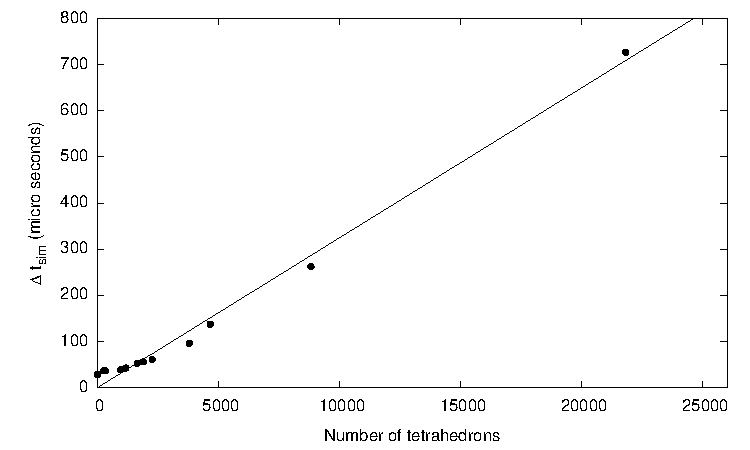
\includegraphics[width=140mm]{./images/results_time_contra_mesh_size.pdf}
  \caption{Graph of the mesh size contra simulation time.}
  \label{fig:time-contra-mesh-size-graph}
\end{figure}

Using the best-fit tool from GNU
Plot\footnote{\url{http://www.gnuplot.info/}} the relation between
simulation time and number of elements can be approximated with a
straight line ($y = \alpha \ x$), where $\alpha \approx 0.032$
with a standard asymptotic error of $2.619\%$.
%
%
% A line has been fitted to the data, which shows how the data develop
% assuming linear
% dependency ($y = \alpha \ x$). Where $\alpha = 30.8436$ with and error
% estimate of $0.7796 = 2.528\%$ using
% GNU Plot.
%
% Next we plot $\Delta t_{sim}$ as a function of the number of nodes,
% this is shown in figure
% \vref{fig:time-contra-number-of-nodes-graph}.
%
% \begin{figure}
%   \centering
%   \includegraphics[width=140mm]{./images/results_time_contra_number_of_nodes.pdf}
%   \caption{Graph of simulation time contra the number of nodes.}
%   \label{fig:time-contra-number-of-nodes-graph}
% \end{figure}
%
%This line have $\alpha=9.01257$, with error estimate of $0.2678 = 2.971\%$.
%
The graph clearly shows that we have a linear dependence
between the geometry size and the time it takes to execute an iteration
of the finite element solver. We expect this linear dependence to hold until
the mesh data exceeds the memory limit of the graphics card.

% \subsection{Scaling the model}
% forklar, floating point presition
% how large can they be: test med graph over presition på shape function
% how small: test med volume = 0

\section{Real-time Analysis}
\label{sec:realtime_analysis}
As stated in section \vref{sec:precompuations}, we have a stability
requirement on the governing equation. The requirement imposes a
critical time step limit, denoted $\Delta t_{cr}$, which must
be met for the system to be stable.
%
This means that the times step we use to iterate the finite element
solver must be smaller than $\Delta t_{cr}$, for the solution to be
stable.
%
If we also want the finite element solver to run in real-time, we must
compute one iteration of the solver than $\Delta t_{cr}$.
%
The conclusions is: If we want the finite element solver to be
stable and run in real-time, then we must have:
$\Delta t_{sim} \le  \Delta t_{cr}$.
%
%
From the critical time step $\Delta t_{cr}$ calculated by equation
\eqref{eq:delta-t-cr} on page \pageref{eq:delta-t-cr} we
obtain:

% The equations for calculating $\Delta t_{cr}$ is defined in equation
% \eqref{eq:delta-t-cr} and \eqref{eq:p-wave-modulus} and is repeated
% below for convenience:

\begin{equation*}
\Delta t_{cr} = \sqrt{\frac{1}{c^2}} L_e = \alpha L_e
\end{equation*}

\begin{equation*}
\frac{1}{c^2} = \frac{\rho}{M}
\qquad \qquad
M = \frac{E(1-\nu)}{(1+\nu)(1-2\nu)}
\end{equation*}

As seen in the equations $\Delta t_{cr}$ is a function of the three
material parameters: $E$, $\nu$, and $\rho$.
%
$\Delta t_{cr} = \alpha L_E$ describes $\Delta t_{cr}$ as a function
of the minimum edge length $L_e$ in the
model.
% One might think that a larger time step could be generated by
% scaling the entire model hereby increasing $L_e$. But since scaling
% the model would increase the weight which then needs to be adjusted by
% lowering the density $\rho$ the two parameters cancel out resulting in an
% unchanged critical time step.
%
%  This is not true because $\alpha$
% contains $\rho$, which also needs to be adjusted when scaling the
% model.
%
In the following example we use the material parameters for dentin.
Teeth are primarily made of dentin which basically consists of
calcium, phosphorus and mineral salts. Dentin is considered a
brittle material since it has very little tendency to deform before
fracturing.
%
%
% as the material
% If we want to calculate $\Delta t_{cr}$ then we need to chose a
% material.
%
% Because a tooth mostly consist of dentin, we chose to use this
% material.
%
By calculating the P-Wave modulus $M$, and $\alpha$ for dentin, where
$E=12 \ GPa$, $\nu=0.32$, and $\rho=2580 \ kg/m^3$ as listed in section
\vref{sec:test-materials} in appendix \appref{chapter:test_data}, we obtain:

% \begin{equation}
% M = \frac{12GPa \cdot (1-0.32)}{(1+0.32)(1-2 \cdot 0.32)}
% = 12 GPa \frac{425}{297} = \frac{1700}{99} GPa
% \approx 17.17 GPa
% \end{equation}

\begin{equation}
M = \frac{12 \cdot (1-0.32)}{(1+0.32)(1-2 \cdot 0.32)}
\approx 17.17 \ GPa
\end{equation}

% \begin{equation}
% \begin{aligned}
% \beta &= \frac{\rho}{M}
% = \frac{2580 \frac{kg}{m^3}}{\frac{1700}{99} G \frac{N}{m^2}}

% = \frac{99 \cdot 2580 \frac{kg}{m}}{1700 G N}
% = \frac{255420 \frac{kg}{m}}{1700 G \frac{kg \cdot m}{s^2}}
% = \frac{255420 \frac{1}{m}}{1700 G \frac{m}{s^2}} \\
% &= \frac{255420}{1700 G \frac{m^2}{s^2}}
% = \frac{12771}{85 G} \frac{s^2}{m^2}
% \approx 150.247 G^{-1} (\frac{s}{m})^2
% = 150.247 \cdot 10^{-9} (\frac{s}{m})^2
% \end{aligned}
% \end{equation}

\begin{equation}
\begin{aligned}
\frac{1}{c^2} &= \frac{\rho}{M}
= \frac{2580 \frac{kg}{m^3}}{\frac{1700}{99} G \frac{N}{m^2}}
\approx 150 \cdot 10^{-9} (\frac{s}{m})^2
\end{aligned}
\end{equation}

% \begin{equation}
% \alpha = \sqrt{\beta}
% = \sqrt{\frac{12771}{85 \cdot 10^{-9}}}
% = \frac{3 \cdot \sqrt{48246}}{1.7 \cdot 10^{6}}
% \approx 387.617 \cdot 10^{-6} \frac{s}{m}
% \end{equation}

\begin{equation}
\alpha = \sqrt{\frac{1}{c^2}}
\approx 387 \cdot 10^{-6} \frac{s}{m}
\end{equation}

Where the units are converted by the following definitions:

\begin{equation}
N = \frac{kg \cdot m}{s^2} \qquad \qquad Pa = \frac{N}{m^2}
\end{equation}

To confirm the dimensions of the tooth, we borrowed an actual
wisdom tooth from the School of Dentistry, Aarhus University, and
modeled this as a mesh in 
millimeters. An axis aligned bounding box around the tooth has the
dimensions: width $\times$ height $\times$ depth,
$10.7 \times 20.1 \times 10.1$.
%
Calculating $\Delta t_{cr}$ for the tooth model, which has a
$L_e= 0.14 \ mm = 0.14 \cdot 10^{-3} \ m$:

\begin{equation}
\Delta t_{cr} = \alpha \cdot L_e
= 387 \cdot 10^{-6}
\cdot 0.14 \cdot 10^{-3}
\approx 55.6 \cdot 10^{-9}s
\end{equation}

which means time progresses with the size of $55.6$ nanoseconds in
each iteration.
%
The constant execution time $\Delta t_{sim}$ for this model, was
measured in section \vref{sec:time-as-a-function-of-geometry} to be
$\Delta t_{sim}= 42.6$ microseconds. This means it takes much more
computational time to predict the next configuration at time $t +
\Delta t$ that the actual time step $\Delta t$ represents. In other
words if it takes $20$ seconds to foresee $10$ seconds into the future
you will always be behind. This illustrates that with the given object
and material properties we cannon achieve real-time performance which
strictly complies with the theoretical laws of physics.

% With the current $\Delta t_{cr}$ we cannot
% accommodate the demand for real-time execution.

\section{The Elasticity Theory}
\label{sec:results_elastic_theory}
In this test scenario we are interested in comparing the simulated
deformation with the theoretical deformation calculated
by hand. The scenario is a beam fixed in one end and stretched by a
displacement modifier in the other end. The direction of the stretch 
is parallel to the $x$-axis. \\

% elasticity
As explained in section \vref{sec:elastic-deformation} elastic
deformation is the physical 
property of a material when it 
deforms due to external forces applied, but returns to its original
shape when the forces are removed. The modulus of elasticity $E$ is used
for defining the elastic property of a given material. The modulus of
elasticity is defined by (equation
\ref{eq:normal_stress_over_normal_strain} on page
\pageref{eq:normal_stress_over_normal_strain}), repeated below:

\begin{equation*}
  E =  \frac{\mbox{normal stress}}{\mbox{normal strain}}
  = \frac{\sigma}{\varepsilon}
  \qquad \Leftrightarrow \qquad
  \varepsilon = \frac{\sigma}{E}
\end{equation*}

As mentioned in section \vref{sec:tled_solver} we use the
Green-Lagrange strain measure $^t_0E_{GL}$ 
with the second Piola-Kirchoff stress measure $^t_0S$ instead of
normal stress and strain. In section \vref{sec:elasticity} we assumed
that the relation between stress and strain is linear since brittle
materials are of our main concern. 
Let us start by measuring the actual
relation between stress and strain to see if the linear assumption is
correct. The following experiments are all conducted with a $20 \times
40 \times 150$ millimeter beam and $E = 12 \ GPa$ corresponding to
dentin. The internal stresses and strains are caused by 
the stretching alone, no other external forces are applied.
The setup is illustrated in figure
\vref{fig:beam_stretching_by_displacement}. Notice how the beam becomes
thinner according to Poisson's ratio as explained in section
\vref{sec:poissons_ratio}.

\begin{figure}
  \begin{minipage}[b]{0.5\linewidth}
    \centering
    \subfloat[]{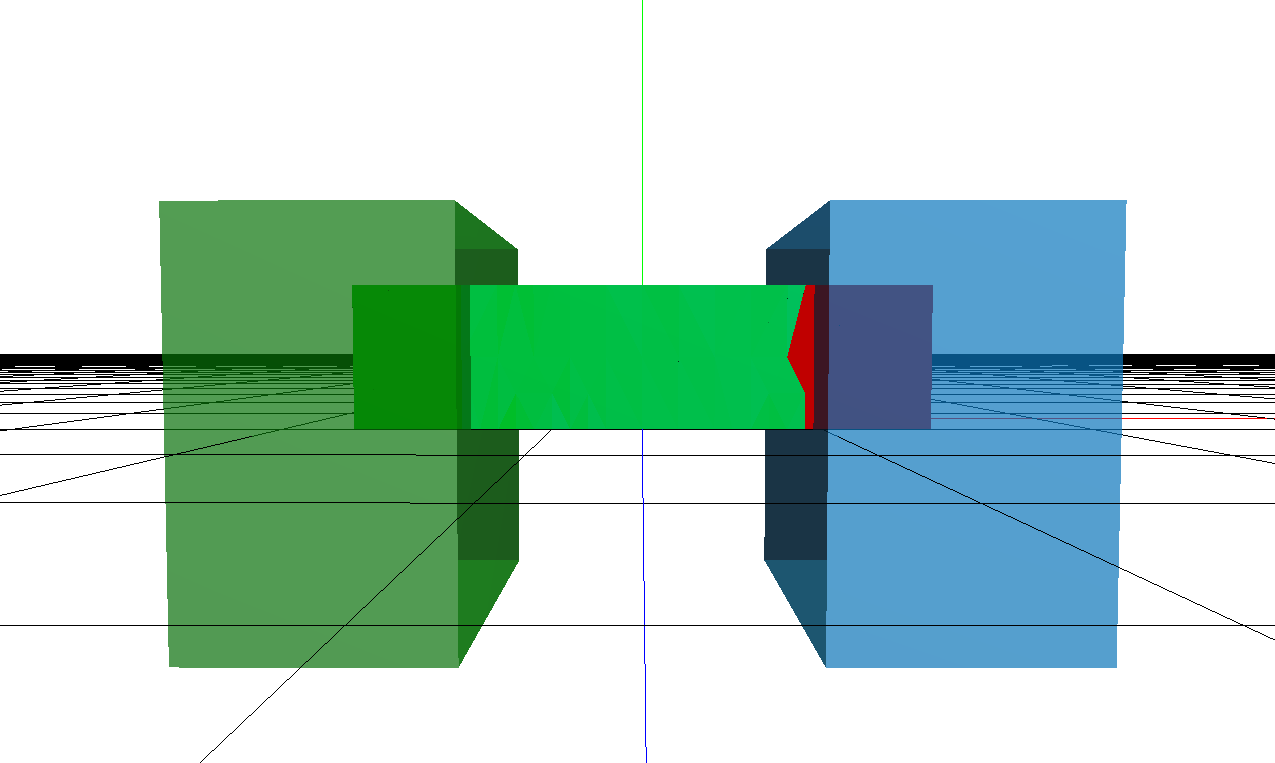
\includegraphics[width=70mm]{./images/results_ssc_displacement_0.png}}
  \end{minipage}
  \begin{minipage}[b]{0.5\linewidth}
    \centering
    \subfloat[]{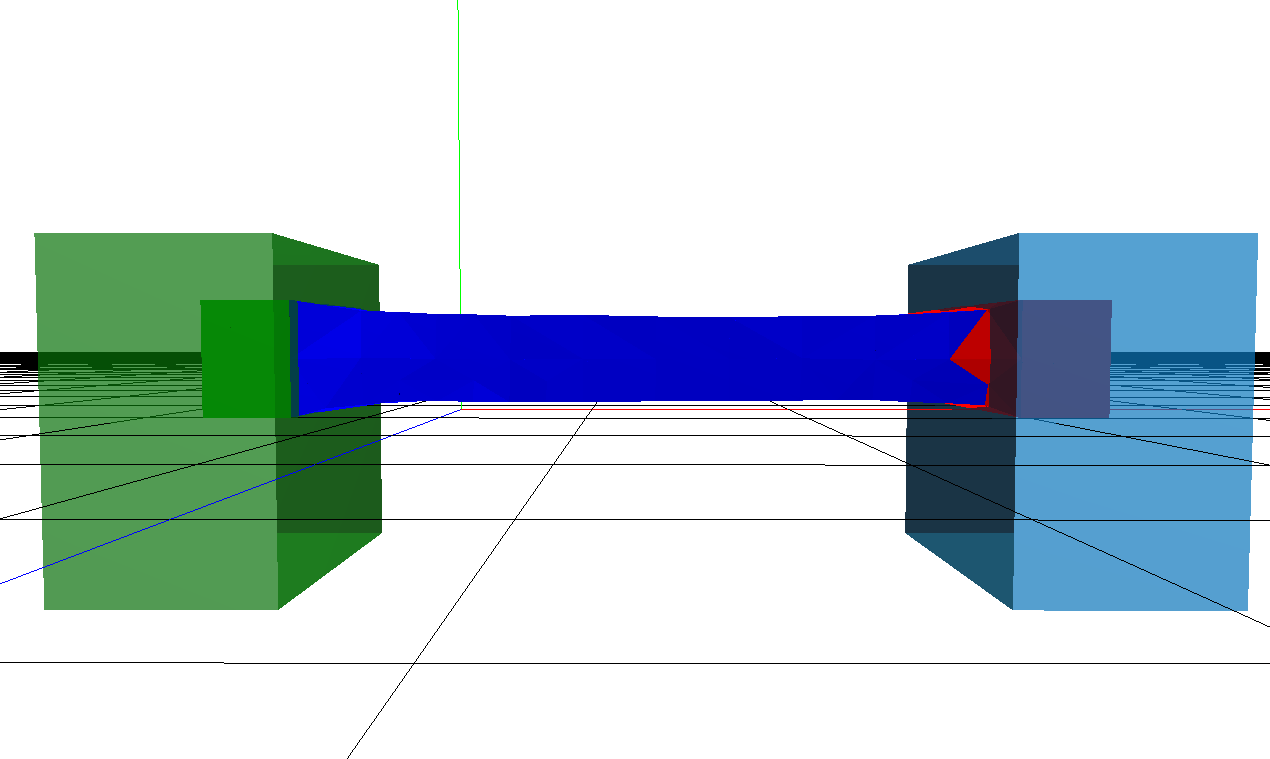
\includegraphics[width=70mm]{./images/results_ssc_displacement_1.png}}
  \end{minipage}
\caption{Beam is being stretched to conduct stress-strain measures.}
\label{fig:beam_stretching_by_displacement}
\end{figure}
  
While the beam is being slowly stretched we measure the Green-Lagrange
strain tensor as defined in equation
\eqref{eq:green_lagrange_strain_tensor} on page 
\pageref{eq:green_lagrange_strain_tensor}:

% Green-Lagrange strain tensor
\begin{equation*}
^t_0E_{GL} = \frac{1}{2}(^t_0C - I)
\end{equation*}

By using the technique described in section
\vref{sec:principal_values_and_directions} we determine the maximum
principal strain value by solving the eigenproblem for the symmetric
tensor $^t_0E_{GL}$. By applying axial stretch along the positive
$x$-direction in the global coordinate frame, the maximum principal
strain direction will also be oriented this way. \\

% measures on the second piola-kirchoff stress tensor
We will now construct a stress-strain curve as the ones introduced in
\vref{sec:sscs}.
It is the maximum principal strain value we are interested in relating
to the maximum principal stress value. The second Piola-Kirchoff
stress measure is used as defined in 
equation \eqref{eq:second_piola_kirchoff_tensor} on page
\pageref{eq:second_piola_kirchoff_tensor}, repeated below:

\begin{equation*}
^t_0S_{ij} = G(\delta_{ij} - ^t_0C_{ij}^{-1}) + \lambda \ ^tJ \ (^tJ-1) \ ^t_0C_{ij}^{-1}
\end{equation*}

Using a similar approach as with the strain value, we solve the
eigenproblem for the symmetric stress tensor $^t_0S$ hereby
determining the maximum principal stress value. The stress and strain
tensors are defined for each tetrahedral element in the body. A random
element located somewhere near the center of the body has been pre-selected.
Once the simulation starts the stress and strain measurements are
conducted every $50^{th}$ iteration. The result is illustrated in
figure \vref{fig:results_stress_strain_curve}.

\begin{figure}
    \centering
    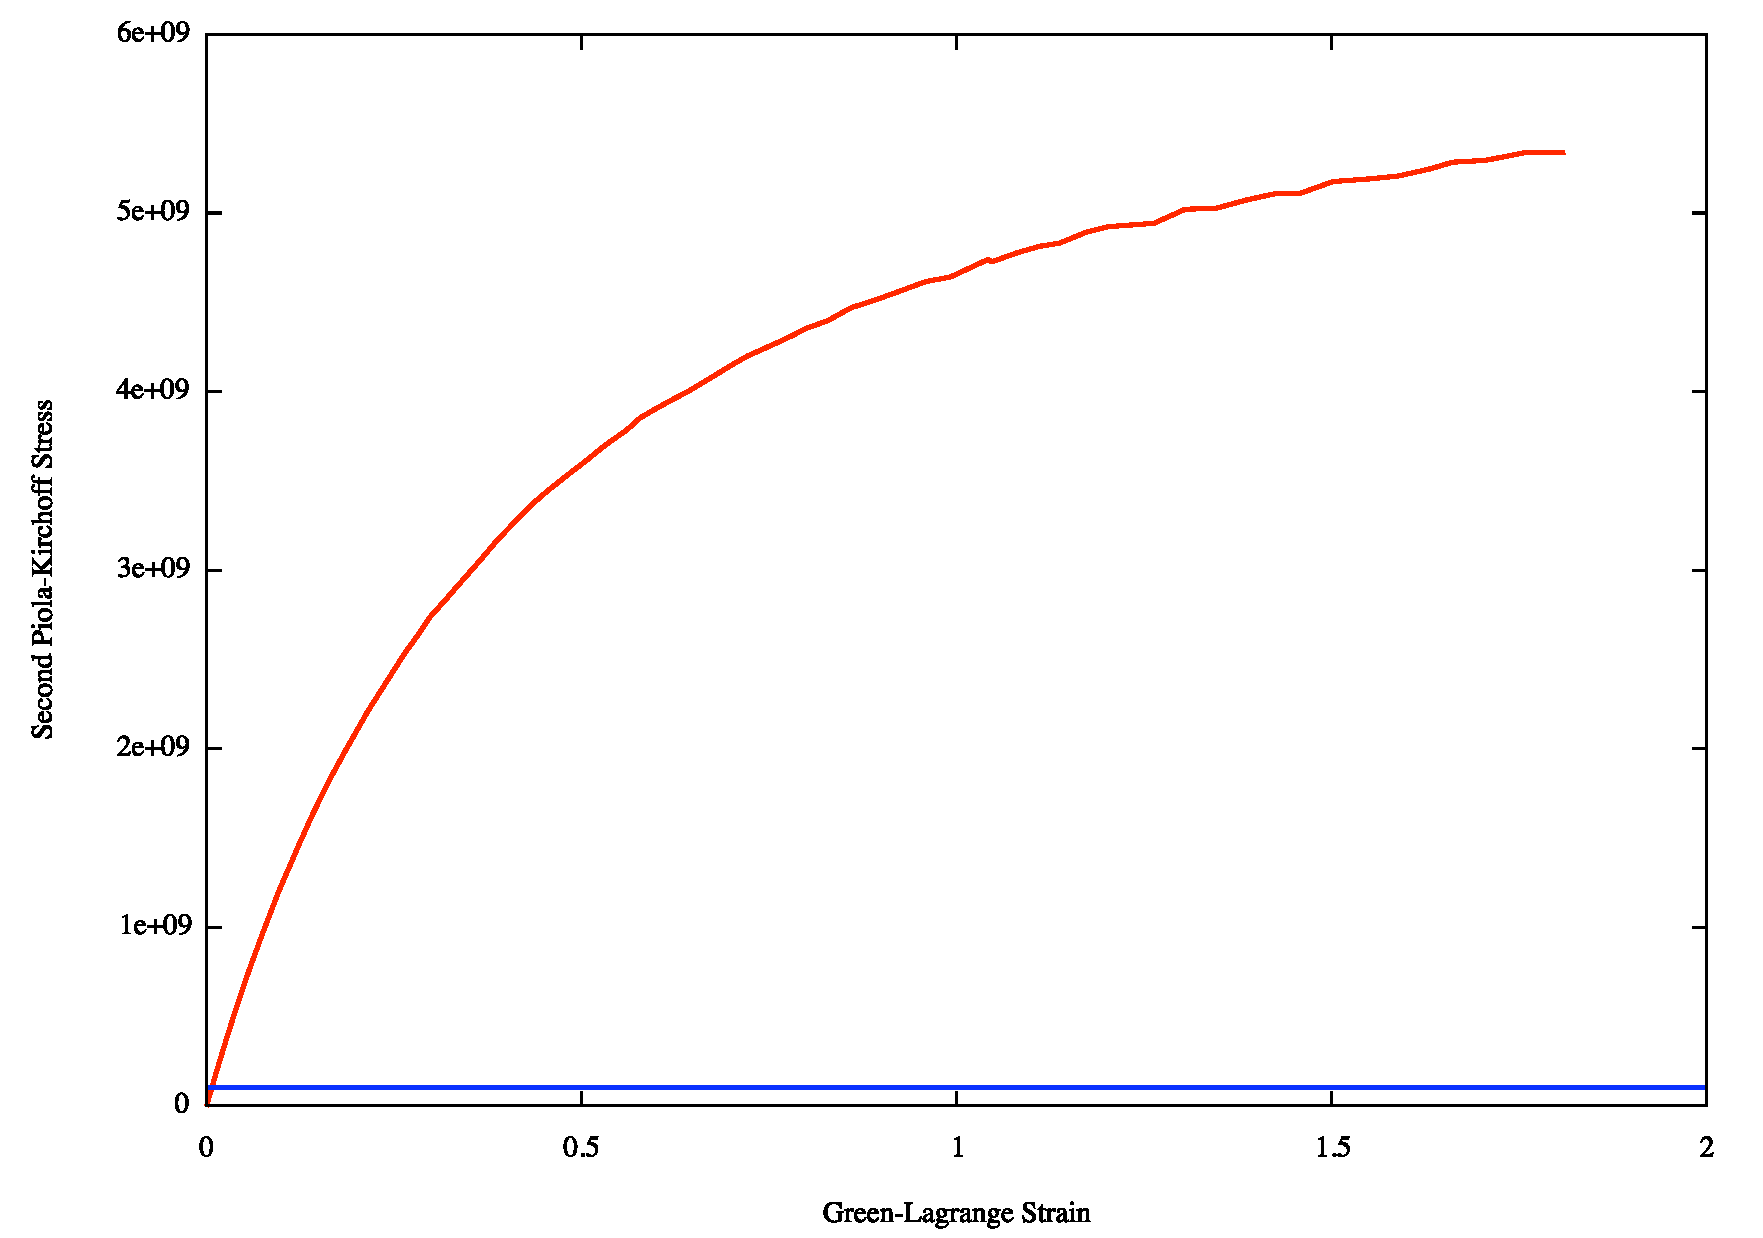
\includegraphics[width=140mm]{./images/results_ssc_dentine_large.pdf}
    \caption{Relation between Green-Lagrange strain and second
      Piola-Kirchoff stress.}
\label{fig:results_stress_strain_curve}
\end{figure}

The relation is obviously non-linear, but as seen on the $x$-axis the
Green-Lagrange strain measure reaches $1.5$. The Green-Lagrange
strain measure is non-linear so physically a measure of $1.5$ means
the beam has been stretched twice its original length. A brittle material like dentin
cannot be stretched this far since its tensile strength is
approximately $100 \ MPa$ ($\sigma^+_F = 100 \times 10^6 \ Pa$)
as described in appendix \appref{chapter:test_data}. The fracturing limit
is illustrated by the horizontal blue line in figure
\vref{fig:results_stress_strain_curve}. 
The maximal strain at the point of fracture is obtained by equation
\eqref{eq:normal_stress_over_normal_strain}:

\begin{align*}
  \varepsilon &= \frac{\sigma^+_F}{E} \vspace{2mm} 
  = \frac{100 \times 10^6}{12 \times 10^9} \vspace{2mm}
  \approx 0.008333
\end{align*}

Considering the $150$ millimeter beam this corresponds to a maximal
stretch of $1.25$ millimeters before the point of fracture is reached.
%
The theoretical elastic modulus $E$ is expressed as a linear relation between
stress and strain. It is reasonable to use the non-linear relation
between the Green-Lagrange strain and the second Piola-Kirchoff stress
in correlation with the linear elastic modulus, because the non-linear
relation is approximately linear below the point of fracture. Figure
\vref{fig:results_stress_strain_curve_closeup} illustrates how close to
linear the simulated relation between stress and strain is.

\begin{figure}
    \centering
    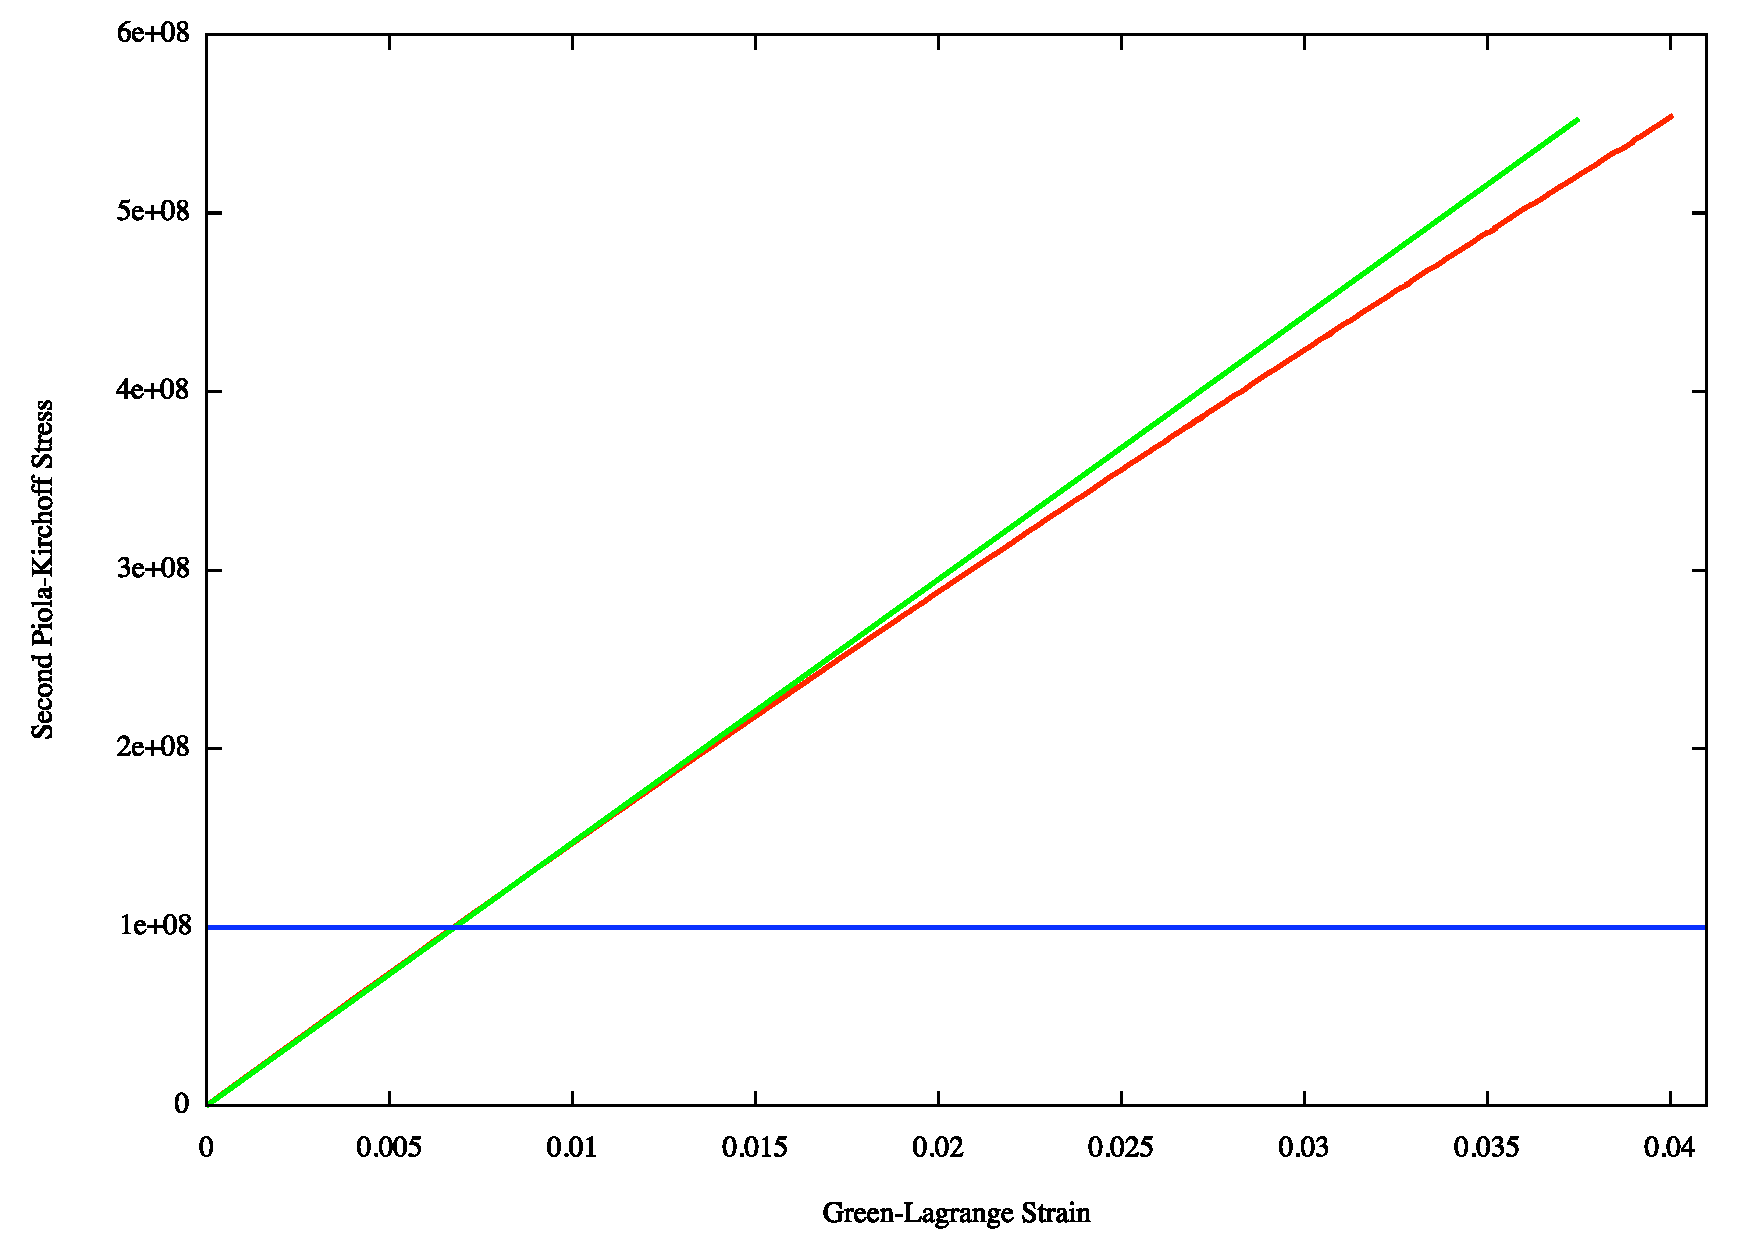
\includegraphics[width=140mm]{./images/results_ssc_dentine_closeup.pdf}
    \caption{Below fracture point the simulated stress-strain relation
      is approximately linear.}
    \label{fig:results_stress_strain_curve_closeup}
\end{figure}

Using the best-fit tool in GNU Plot the measured relation between
stress and strain, below the point of fracture, can be approximated
with a straight (green) line ($y = \alpha \ x$), where
$\alpha = 1.4730 \times 10^{10}$ with a standard asymptotic error of
$0.2\%$.
%
Brittle materials are defined to be materials that can be
model by a linear stress-strain relation (described in section
\vref{sec:brittle-ductile}).
%
As illustrated although we are using the non-linear neo-Hookean
elasticity theory, we have an approximate linear dependence between
stress and strain for brittle materials (dentin) below the fracture
point.

%  \{This illustrates that brittle materials
% can be approximated by the non-linear neo-Hookean elasticity model.}

%
% Even though the point of origin is an
% elastic modulus of $1.2 \times 10^{10}$ the simulated relation in the
% linear area is closer to $1.4730 \times 10^{10}$ which causes an
% margin error of $\approx 22.75\%$ above the theoretical.
%
% which can
% be approximated with a linear relation between stress and strain as
% illustrated by the green line representing the elastic modulus for
% concrete in illustration
% \vref{fig:results_stress_strain_curve}. Depending on the elastic
% modulus the non-linear stress and strain relation can be linear
% approximated at the low end. With concrete we can linearly approximate
% the relation to about a stress of $4 \times 10^9$ (the blue line) which
% corresponds to a 
% Green-Lagrange strain measure of $0.121$ or a body deformation of
% $\approx 11\%$. As the deformation increases so does the error of the
% approximation, right below the blue line the difference between the
% measured and approximated stress is $\approx 15\%$. \\
% As mentioned in the introduction the main concern is to produce
% plausible results on how objects would break due to externally applied
% loads. 


%-------------
% The fracturing algorithm described in section
% \vref{sec:crack_tracking_algorithm} on page
% \pageref{sec:crack_tracking_algorithm} relies on the stress and strain  
% calculations therefore it is interesting to measure the accuracy
% of the simulated physics. We calculate the expected deformation by
% hand and compare this to the measured deformation in the simulation.
% The expected amount of stretch is obtained
% by\citebook{page~10}{book:strength-materials}: 

% \begin{equation}
% \Delta L = \frac{F \cdot L}{A \cdot E}
% \end{equation}

% where $L$ is the length of the beam, $\Delta L$ is the stretch,
% $F$ is the applied force, $A$ is the cross-sectional area, and $E$ is
% the elastic modulus. Using a beam with the
% dimensions $150 \times 40 \times 20$ millimeters an elastic modulus of
% $12$ GPa, and a force of $10^6$ N, we obtain a
% stretch of: 

% \begin{equation*}
% \Delta L = \frac{10^6 N \cdot 150 \ mm}{800 \ mm^2 \cdot 12
% \cdot 10^9 \ N/mm^2}
% \approx 1.5625 \cdot 10^{-5} \ mm 
% \end{equation*}
% \{oleby}{$N/mm^2$?} 

% According to the calculation $10^6 N$ should stretch the
% beam by $1.5625 \cdot 10^{-5}$ millimeters. Simulating a beam with same
% dimensions and the same force results in a stretch of $2.73618 \cdot
% 10^{-5}$, which is $\approx 75.11\%$ above the calculated. Table
% \vref{tab:stretch_results} shows the comparison between calculated and
% measured deformations. \\

% \{oleby}{colunms are to wide in the table} 

% \begin{table}
%  \begin{center}
% \label{tab:stretch_results}
%     \begin{tabular}{c|c|c|c}
%     \hline
%     Force applied (Newton)& $\Delta L$ Calculated (millimeters) & $\Delta
%     L$ Measured (millimeters)& Error (\%)\\ \hline
%     % 
%     $1.0 \cdot 10^6$ & $1.5625 \cdot 10^{-5}$ & $2.73618 \cdot 10^{-5}$ & $75.11$ \\ \hline
%     %
%     $5.0 \cdot 10^6$ & $7.8125 \cdot 10^{-5}$ & $11.7339 \cdot 10^{-5}$ & $50.19$ \\ \hline
%     %
%     $25.0 \cdot 10^6$ & $3.90625 \cdot 10^{-4}$ & $5.98259 \cdot 10^{-4}$ & $53.14$ \\ \hline
%     % 
%     $50.0 \cdot 10^6$ & $7.8125 \cdot 10^{-4}$ & $11.9082 \cdot 10^{-4}$ & $52.42$ \\ \hline
%     %
%     $100.0 \cdot 10^6$ & $1.5625 \cdot 10^{-3}$ & $2.3761 \cdot 10^{-3}$ & $52.07$ \\ \hline
%     \end{tabular}
% \end{center}
%    \caption{Table showing the comparison between calculated and measured
%       deformation.}
% \end{table}

% As seen in table \vref{tab:stretch_results} the margin of error 
% seems approximately constant except
% for the first measurement where the expected deformation is so small
% its reasonable
% to expect significant numerical errors in addition to all the other
% approximations made throughout the calculations (e.g. by the explicit
% time integration).\{oleby}{???}
%------------------- 

\section{Fragmentation of Supported Beam}
This is the first scenario with the purpose of testing the crack tracking
algorithm. The main purpose is to see if the crack tracking algorithm
determines a failure surface according to our intuition of
how the concrete beam would break. The scenario is simple; a beam is
located the top of two boxes supporting each end of the beam as
illustrated in figure \vref{fig:double_supported_beam_0}. A third
box is slowly being moved downwards hereby forcing on top of the beam
down until the beam fractures. Concrete is considered a brittle
material so the beam is expected to fracture vertically somewhere
around its center where the internal forces will peak. 

\begin{figure}
  \begin{minipage}[b]{0.5\linewidth}
    \centering
    \subfloat[]{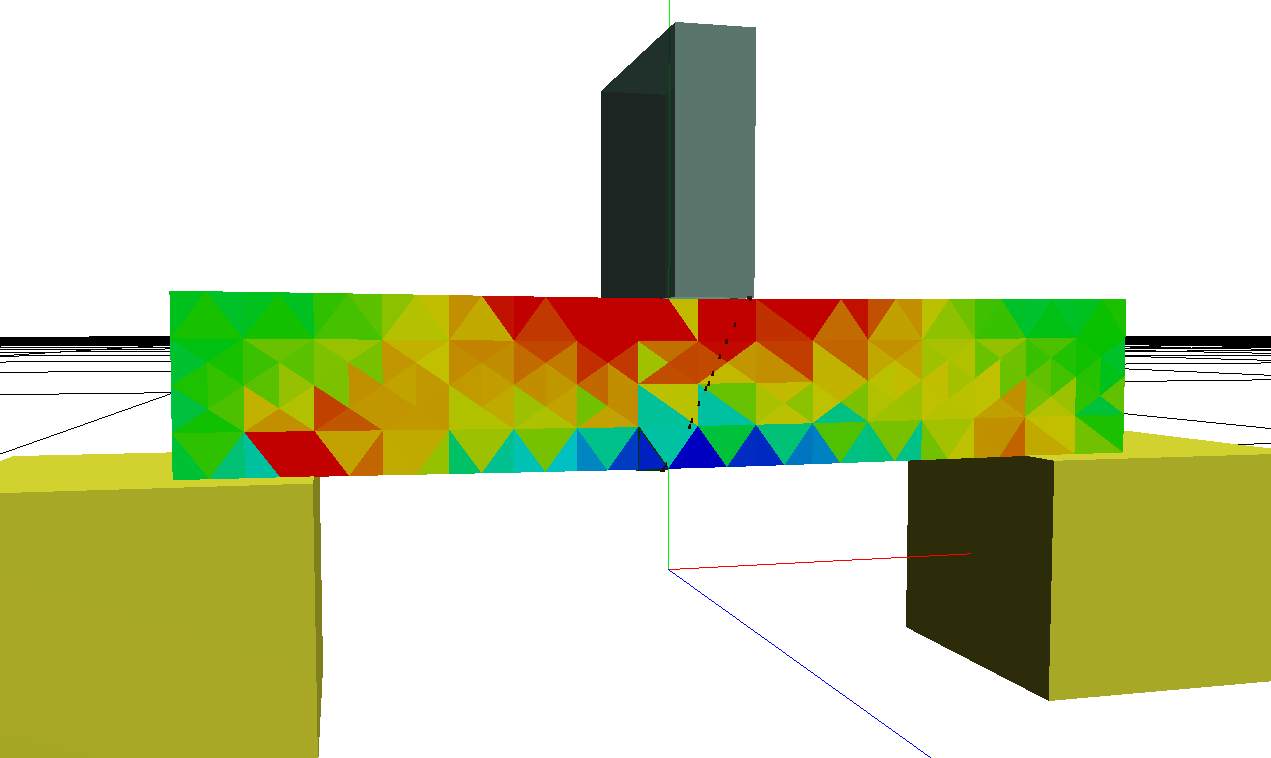
\includegraphics[width=70mm]{./images/results_double_supported_beam_0.png}
    \label{fig:double_supported_beam_0}}
  \end{minipage}
  \begin{minipage}[b]{0.5\linewidth}
    \centering
    \subfloat[]{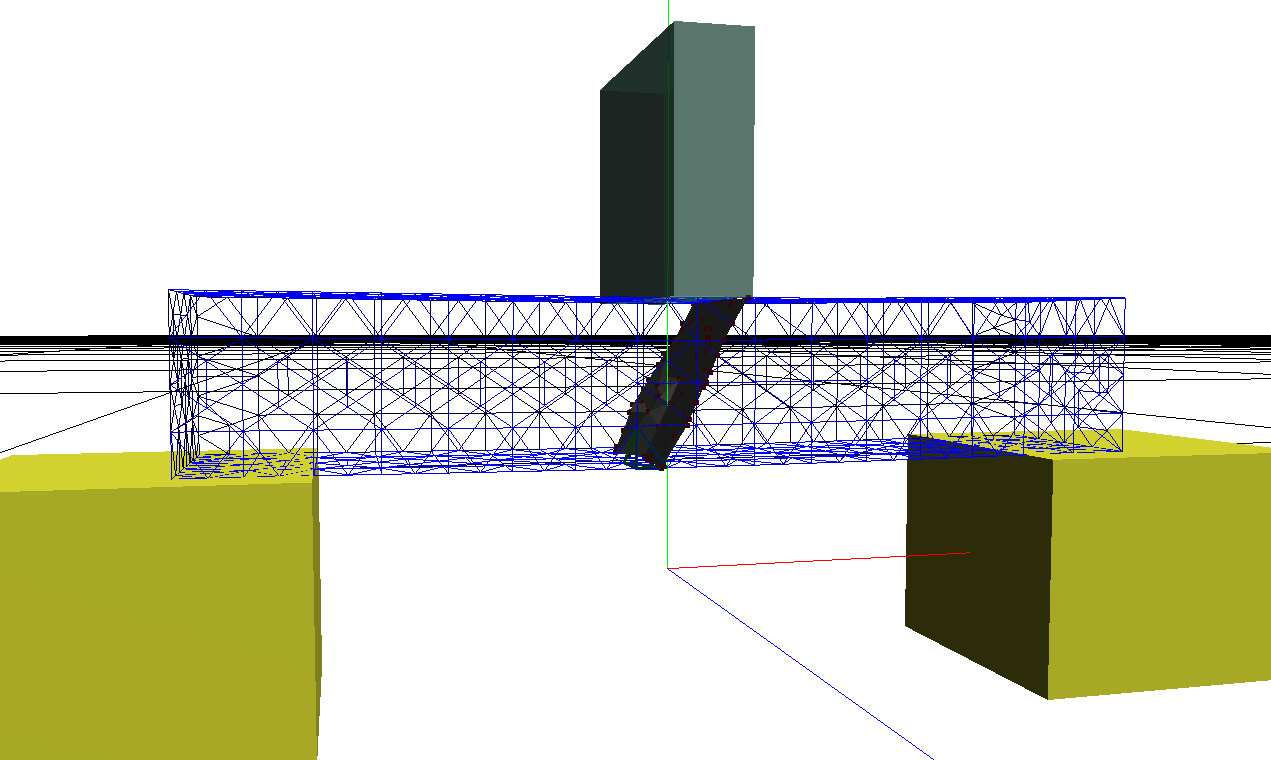
\includegraphics[width=70mm]{./images/results_double_supported_beam_1.png}
    \label{fig:double_supported_beam_1}}
  \end{minipage}
\caption{Fragmentation of supported beam.}
\label{fig:double_supported_beam}
\end{figure}

The beam bends as the force increases gradually causing the internal
stress to peak around the center of the beam. As seen on
\vref{fig:double_supported_beam_0} the beam is compressed on the top
and stretched at the bottom peaking around the center.
When the material dependent point of fracture ($\sigma^-_F$ or $\sigma^+_F$) is exceeded the crack is
initialized and starts to propagate through the solid object. As
illustrated in figure \vref{fig:double_supported_beam_1} the crack
tracking algorithm determines a failure surface located around the
center of the beam propagating vertically as expected. At the top of
the beam the failure surface is located slightly to the right of where
the external forces are applied. As expected the crack propagates
towards the center of the beam here creating a slightly curved
failure surface. The point of origin and the
curvature depends on the amount of force being applied and especially
the rate at which they are applied. 


\section{Mesh Independent}
When it comes to approximating the shape of an object the number of
elements determines the quality of the approximation. As explained in
section \vref{sec:discretize-the-continuum} any solution domain with curved
boundaries can be approximated by a series of straight lines or flat
planes. When discretizing a complex shaped object we must
choose an appropriate element size in order to make a reasonable
approximation. This is not the case with simple
shaped objects like a beam. It is a rectangular box which can be
discretized by a minimum of five tetrahedra as illustrated in figure
\vref{fig:hexahedron2tetrahedra}.
%
Discretizing a beam into five elements would probably not be advisable
due to the quality of the failure surface.
A minimum of five
elements are enough for approximating the shape but not for a
reasonable approximation of the failure surface. In general we are
interested in how the number of elements, hence the quality of the
mesh, affects the outcome of the crack tracking algorithm. 
For benchmark purposes we have constructed four beams with the exact
same dimensions but with gradually increasing number of elements as
described in section \vref{sec:bar-mesh} in appendix \ref{chapter:test_data}.
The beam is fixed in one end while external forces are
applied at the other end. The external forces pulling down are 
uniformly distributed on the selected nodes (elements colored
gray). Each beam 
setup is exactly the same, illustrated in figure
\vref{fig:mesh_beam_setup}.

\begin{figure}
    \centering
    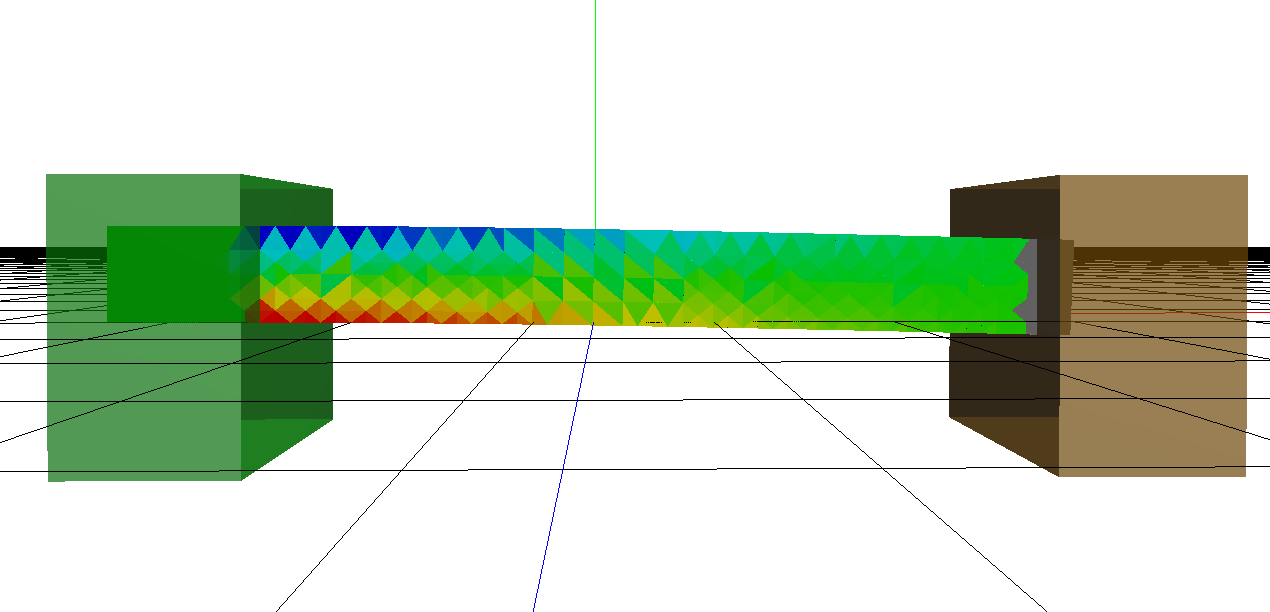
\includegraphics[width=100mm]{./images/results_mesh_setup.png}
    \caption{Benchmark setup for testing mesh dependency.}
    \label{fig:mesh_beam_setup}
\end{figure}

Each beam was tested one at the time and as seen on figure \vref{fig:mesh_beam_results}
the resulting failure surfaces determined by the crack tracking
algorithm are fairly similar. In all four cases the point of origin of
the crack was located slightly to the right of the supported area and the
orientation of the initial crack plane was vertical. Although the four
failure surfaces are slightly different they are all equally located
and oriented. By increasing the mesh quality we also increase the
number of crack planes and hereby the details in the continuous failure
surface. As seen on figure \vref{fig:mesh_beam_results_3} the failure
surface is more curved than on figure \vref{fig:mesh_beam_results_0}
but the overall location and vertical curvature remains the same.
In this scenario the crack tracking algorithm and the failure surface
determined seems unaffected by the increasing quality of the mesh.
 
\begin{figure}
  \begin{minipage}[b]{0.5\linewidth}
    \centering
    \subfloat[Beam with 263 elements.]{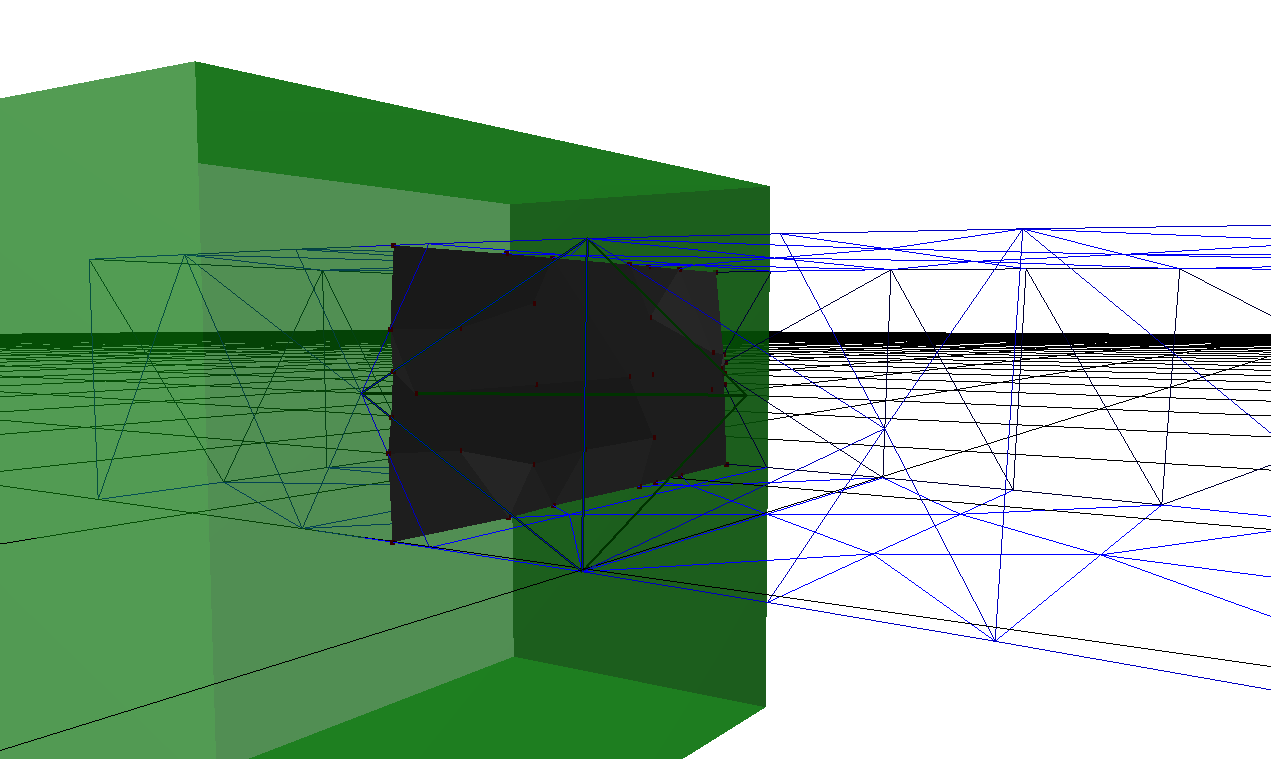
\includegraphics[width=65mm]{./images/results_mesh_bream_crack0.png}
  \label{fig:mesh_beam_results_0}}
  \end{minipage}
%  \hspace{0.5cm}
  \begin{minipage}[b]{0.5\linewidth}
    \centering
    \subfloat[Beam with 964 elements.]{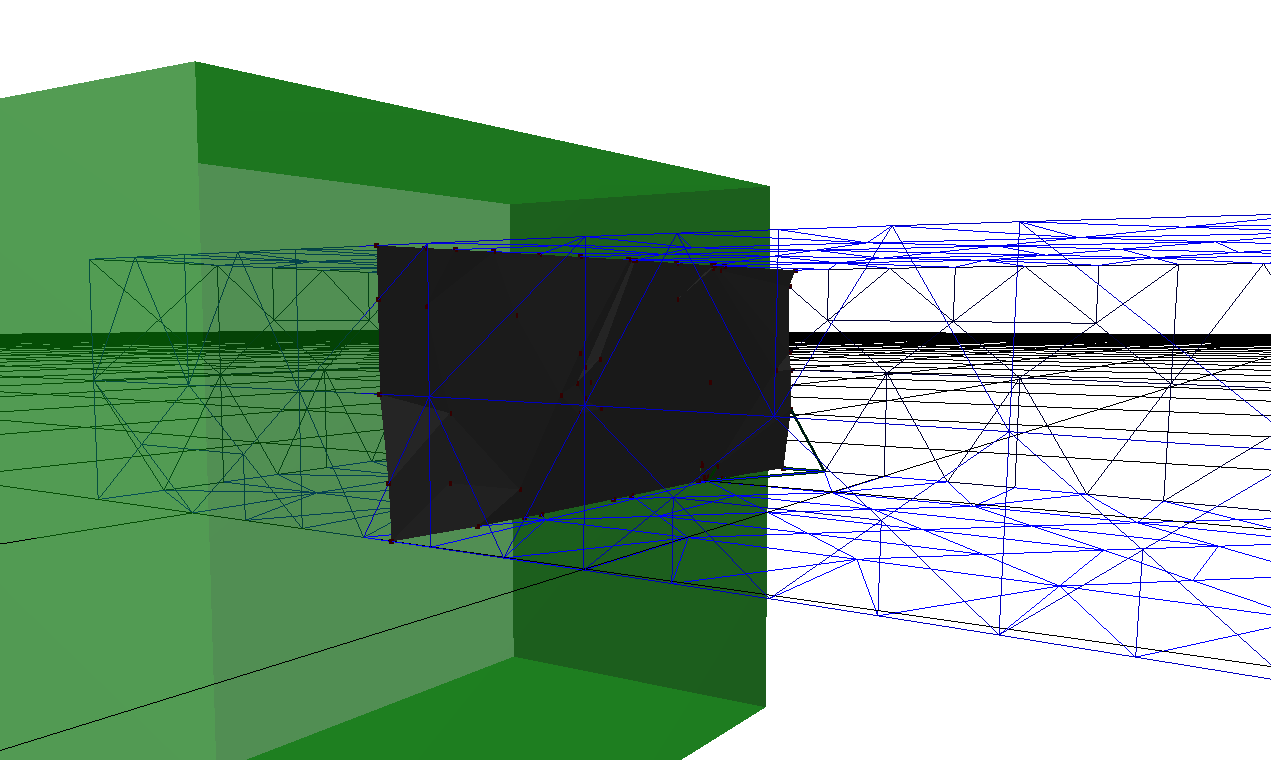
\includegraphics[width=65mm]{./images/results_mesh_bream_crack1.png}}
  \end{minipage}
  \newline
  \begin{minipage}[b]{0.5\linewidth}
    \centering
    \subfloat[Beam with 4658 elements.]{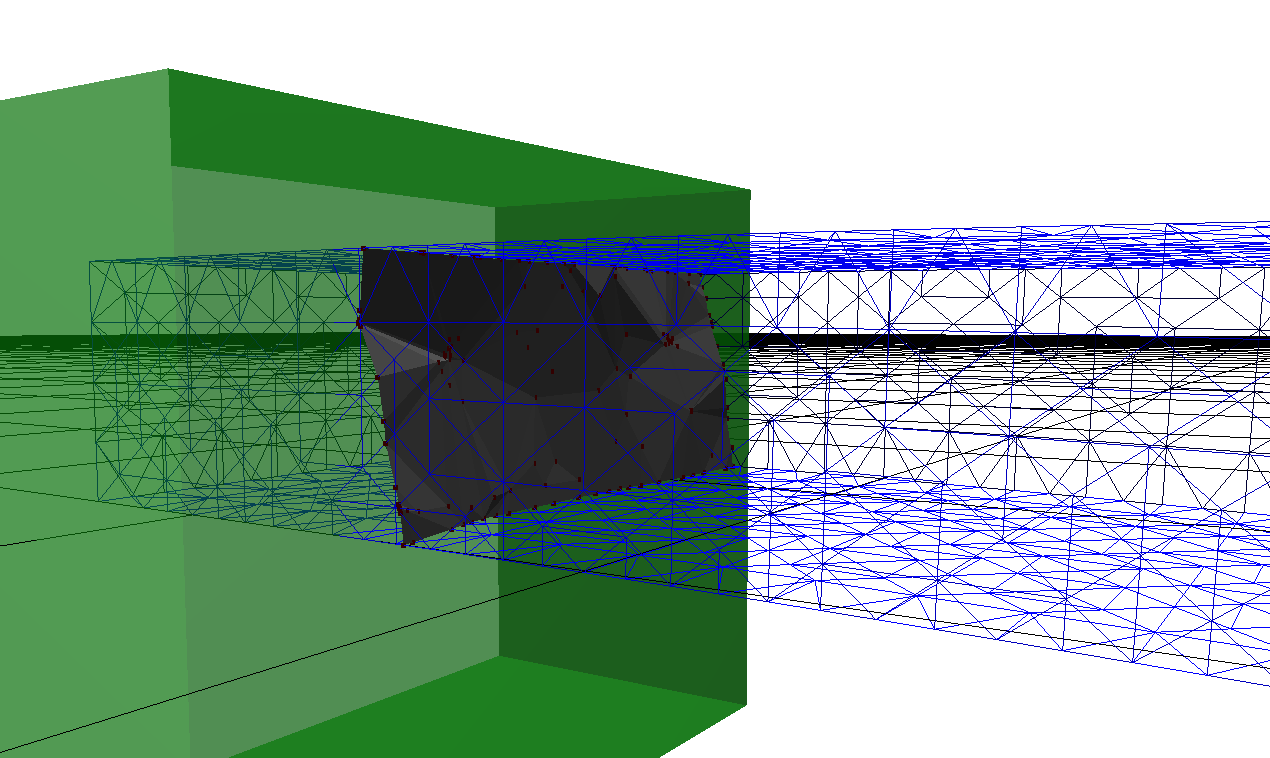
\includegraphics[width=65mm]{./images/results_mesh_bream_crack2.png}}
  \end{minipage}
 % \hspace{0.5cm}
  \begin{minipage}[b]{0.5\linewidth}
    \centering
    \subfloat[Beam with 21809 elements.]{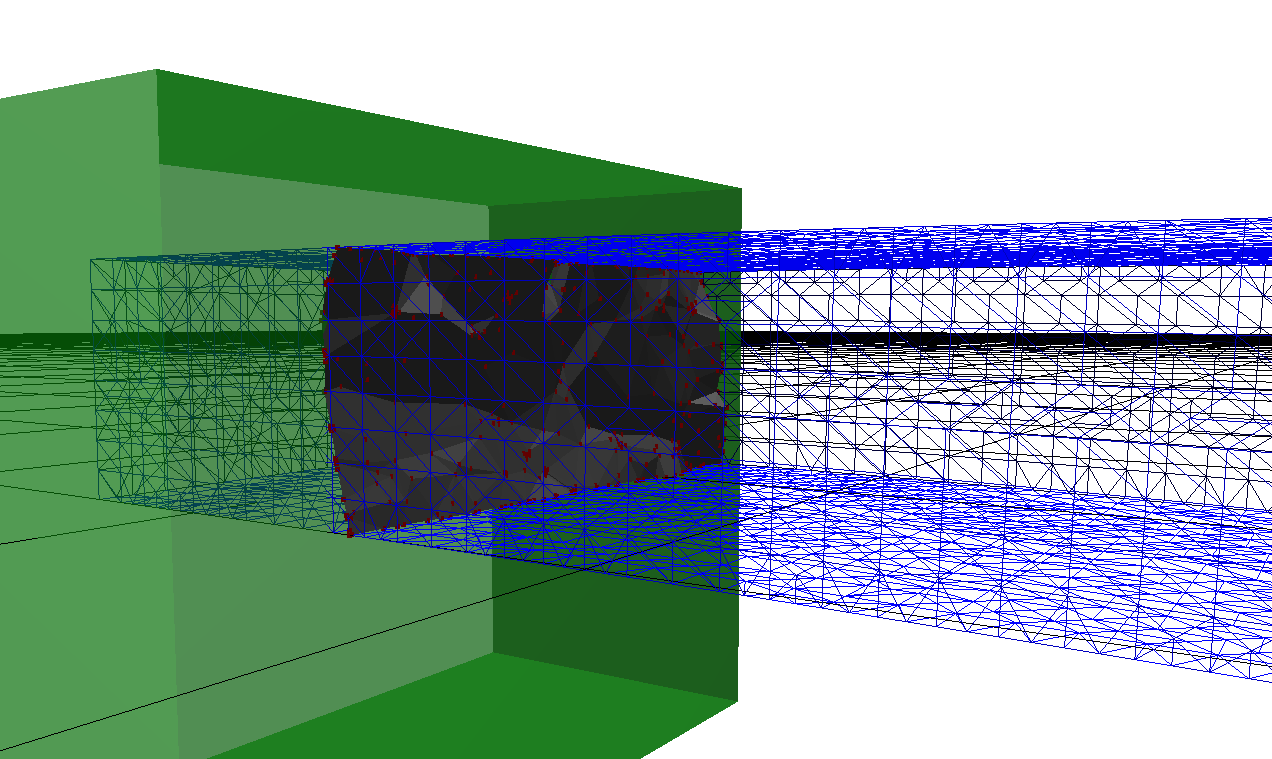
\includegraphics[width=65mm]{./images/results_mesh_bream_crack3.png}
  \label{fig:mesh_beam_results_3}}
  \end{minipage}
  \caption{Crack tracking with beam in different mesh qualities.}
  \label{fig:mesh_beam_results}
\end{figure}



\section{Fragmentation of Tooth Mock-up}
The purpose of this scenario is once again to see if the crack
tracking algorithm determines a failure surface according to our
intuition. The solid object being used in this scenario is a mock-up
of a tooth with a groove drilled halfway through. Due to the groove
the object must be weakened in this area and is therefore expected to
fracture somewhere close to this. The bottom of the tooth mock-up is fixed
while forces are being applied gradually at the top pushing the object
to the right. Again we use dentin as the material ($E = 12 GPa$):

\begin{figure}
  \begin{minipage}[b]{0.5\linewidth}
    \centering
    \subfloat[]{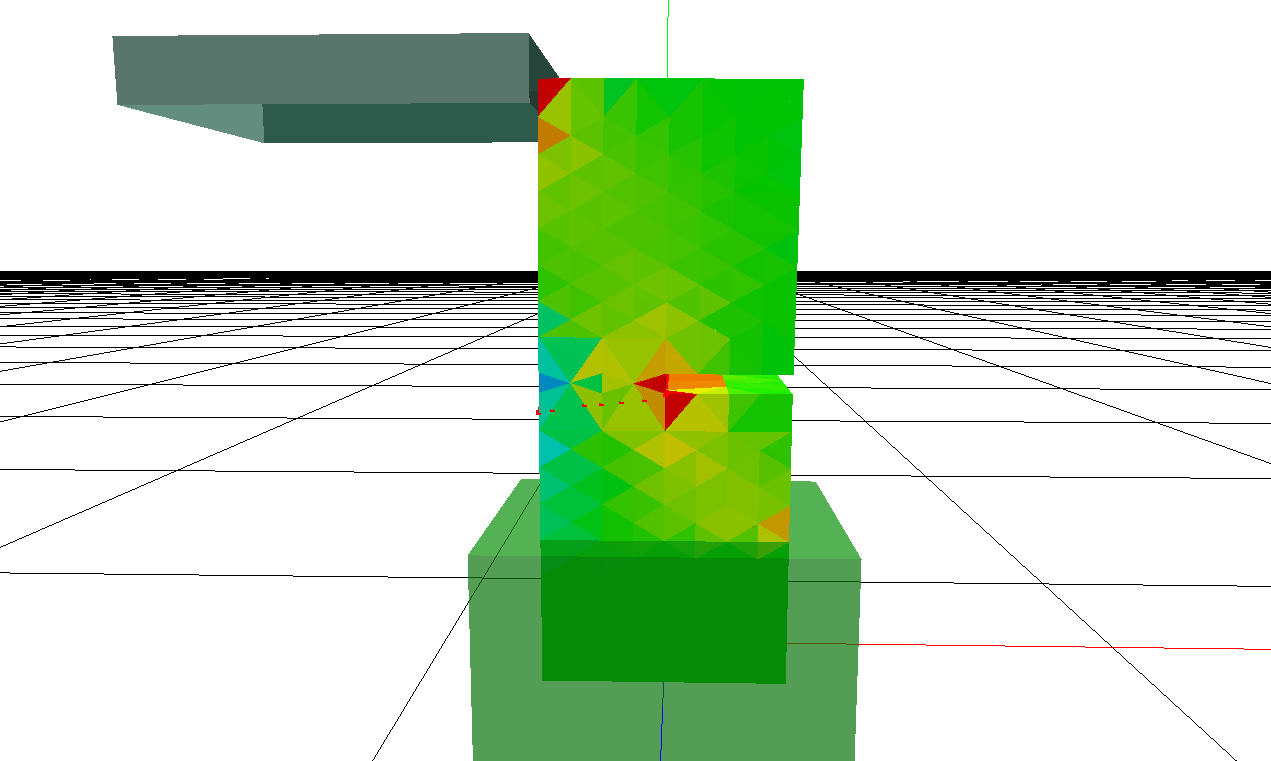
\includegraphics[width=70mm]{./images/results_tooth_mock_up_0.png}
  \label{fig:tooth_mock_up_0}}
  \end{minipage}
  \hspace{0.5cm}
  \begin{minipage}[b]{0.5\linewidth}
    \centering
    \subfloat[]{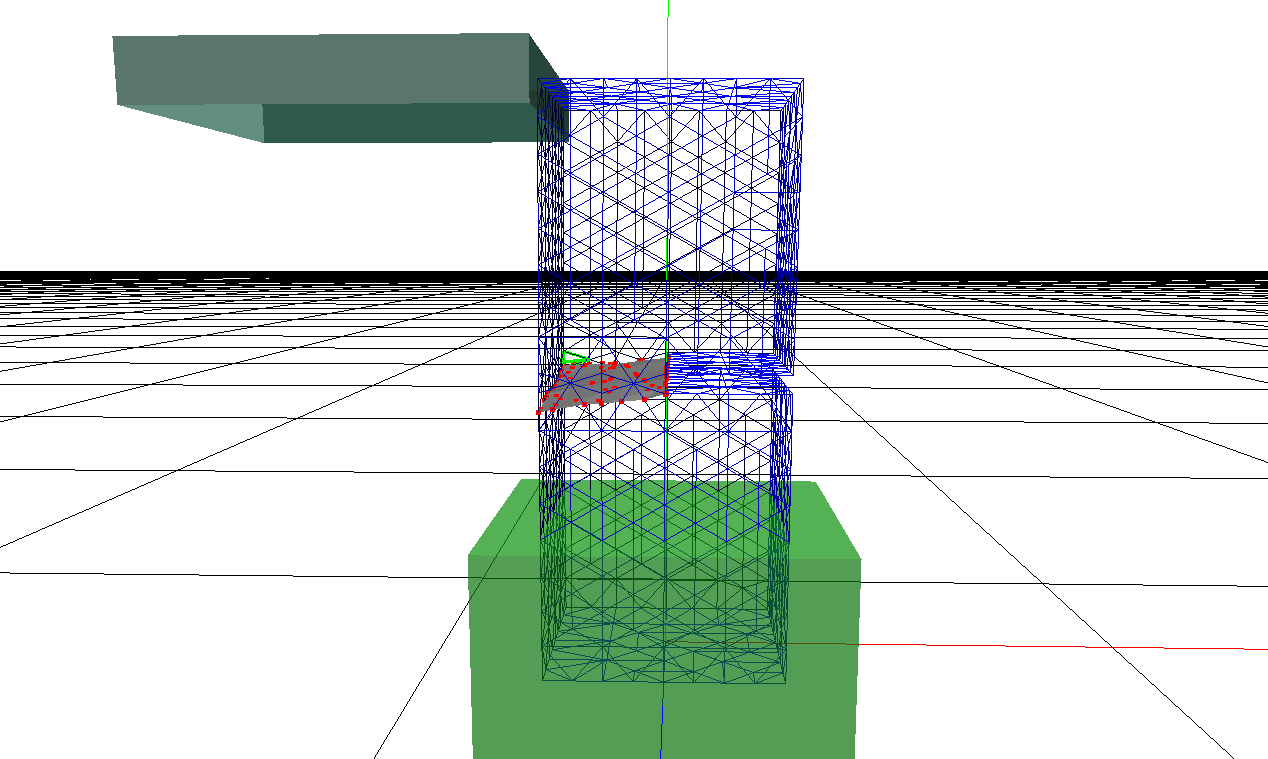
\includegraphics[width=70mm]{./images/results_tooth_mock_up_1.png}
  \label{fig:tooth_mock_up_1}}
  \end{minipage}
  \caption{Fragmentation of tooth mock-up.}
  \label{fig:tooth_mock_up}
\end{figure}

As seen on figure \vref{fig:tooth_mock_up_0} the modifier pushes the
top of the tooth mock-up to the right, which causes compression near 
the groove. The pressure is gradually increased until the point of
fracture ($\sigma^-_F$ or $\sigma^+_F$) is exceeded. The failure
surface as seen on figure \vref{fig:tooth_mock_up_1} started at the
bottom of the groove and propagated to the left slightly curving
downwards. The beam is fragmented around its weak midpoint near the groove
as expected.    

\layoutnewpage

\section{Fragmentation of Tooth}
\label{sec:results_fragmentation_tooth}
In this scenario a tooth model is fragmented using a
simulated dental tool known as an elevator, as depicted
in figure \vref{fig:elevator}. When the
groove has been drilled in the 
tooth, the elevator is inserted into the groove and twisted in order
to deform the brittle dentin material just enough to cause
fracture. The tip of the elevator tool is actually slightly curved
which makes it suitable for elevating both the crown and the roots
once they are separated. In this scenario attention is only focused on fracturing the
tooth and not on how to elevate the separated parts from the
jawbone. The representation of the elevator tool is therefore
simplified to a non-curved plane as illustrated in figure
\vref{fig:tooth_fracture_setup}. The tooth model is fixed by its roots
similar to the actual scenario. Performing the drilling of the groove
is beyond the scope of this simulator, therefore the tooth model has a
predefined groove with a depth that corresponds to $1/3$ of the
tooth's width. 

\begin{figure}
    \centering
    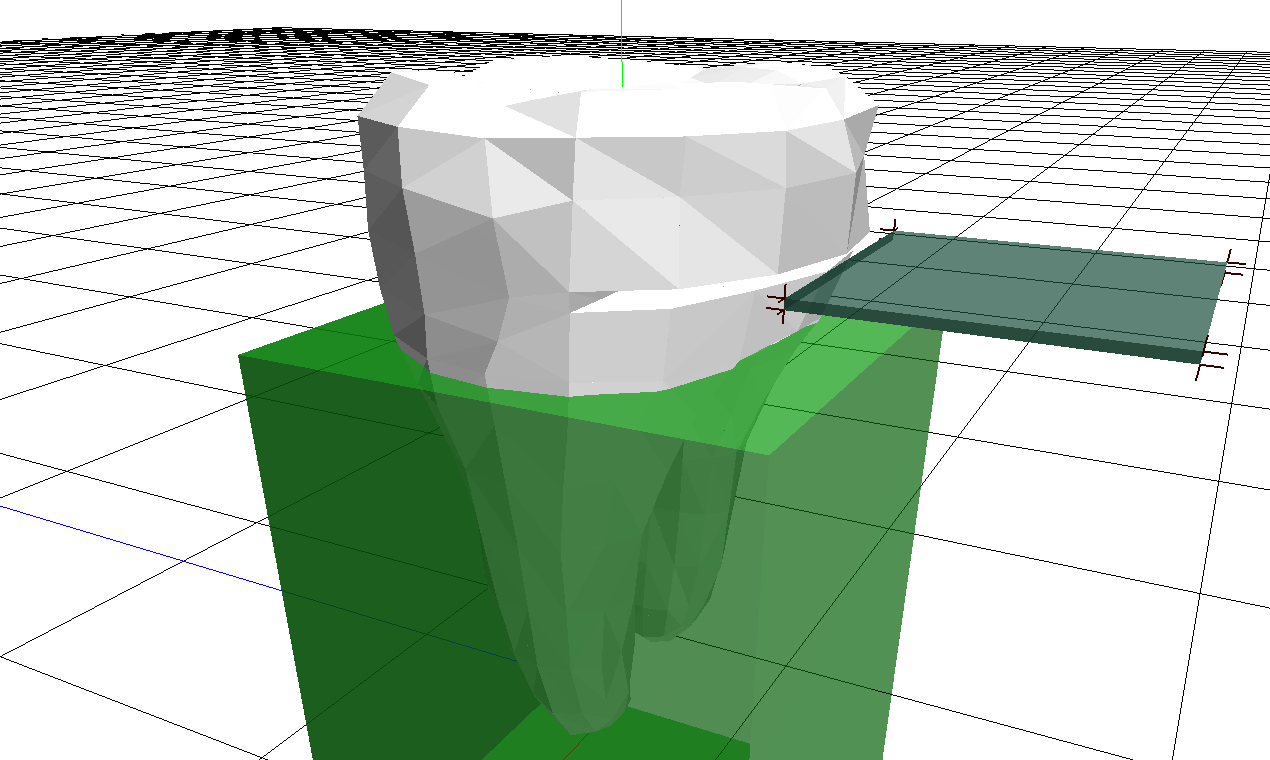
\includegraphics[width=140mm]{./images/results_tooth_fracture_setup.png}
    \caption{The tooth model with a predefined groove.}
    \label{fig:tooth_fracture_setup}
\end{figure}

The elevator tool in inserted into the groove and slowly twisted until
the dentin material has been deformed beyond its fracture
point. External forces are applied in a somewhat different way in
comparison with the other scenarios. Since the elevator tool is twisted
all forces are applied to a relatively small area. When the tool is
twisted the crown is being forced upwards, while the roots
are being forced downwards. The twisting motion of
the elevator tool causes maximum tension at the bottom of the groove
as expected. As seen on figure \vref{fig:tooth_crack_propagation_0} the
crack has its origin at the bottom of the groove. As the crack
propagates in all directions from its origin, the orientation of the
failure surface becomes clear. Due to the restriction on the roots the
only part free to move is the
crown, therefore it slightly tilts backwards
as the groove is gradually being widened. The stress starts to point
downwards on the opposite side of where the groove is located. This
reaction explains why the failure surface tends to curve
downwards eventually reaching the surface of the material slightly
lower compared to the horizontal location of the groove. The curvature of the
failure surface starts to emerge early in the propagation as seen in
figure \ref{fig:tooth_crack_propagation_2}.

\begin{figure}
  \begin{minipage}[b]{0.5\linewidth}
    \centering
    \subfloat[]{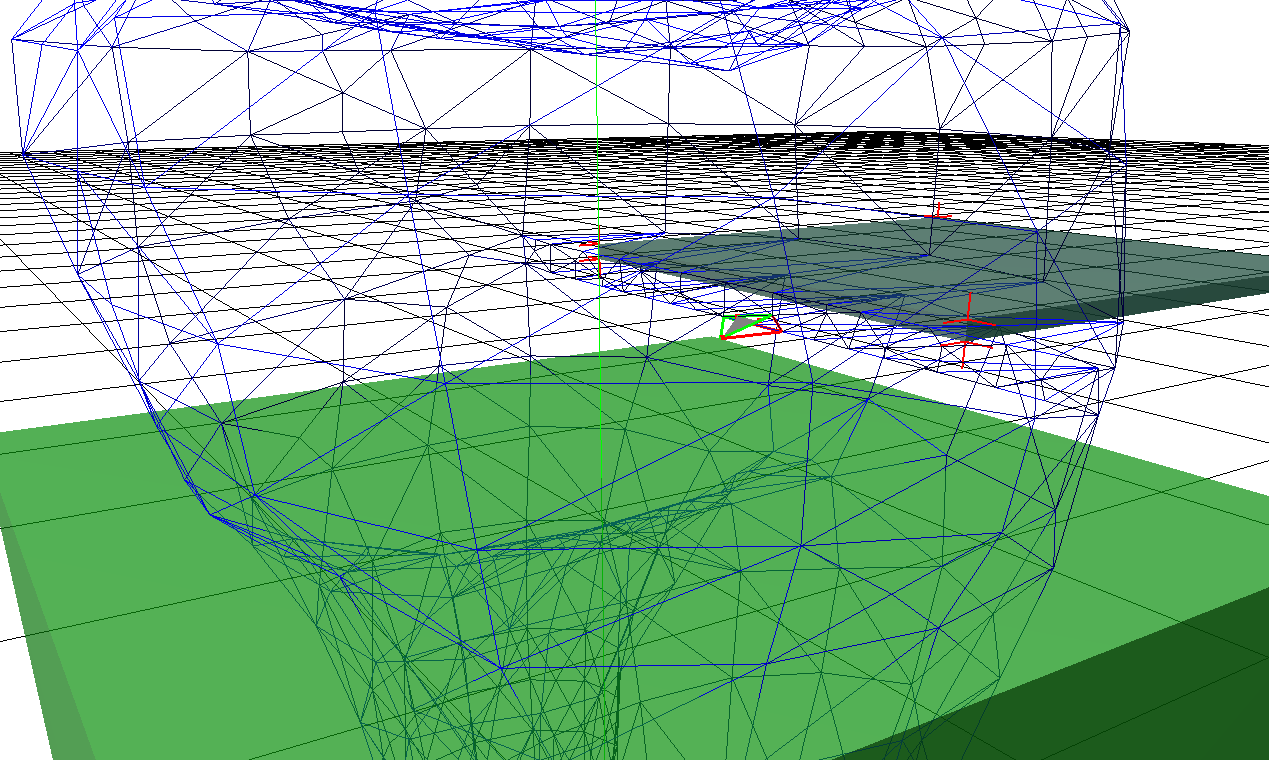
\includegraphics[width=70mm]{./images/results_tooth_fracture_propagation_0.png}
  \label{fig:tooth_crack_propagation_0}}
  \end{minipage}
%  \hspace{0.5cm}
  \begin{minipage}[b]{0.5\linewidth}
    \centering
    \subfloat[]{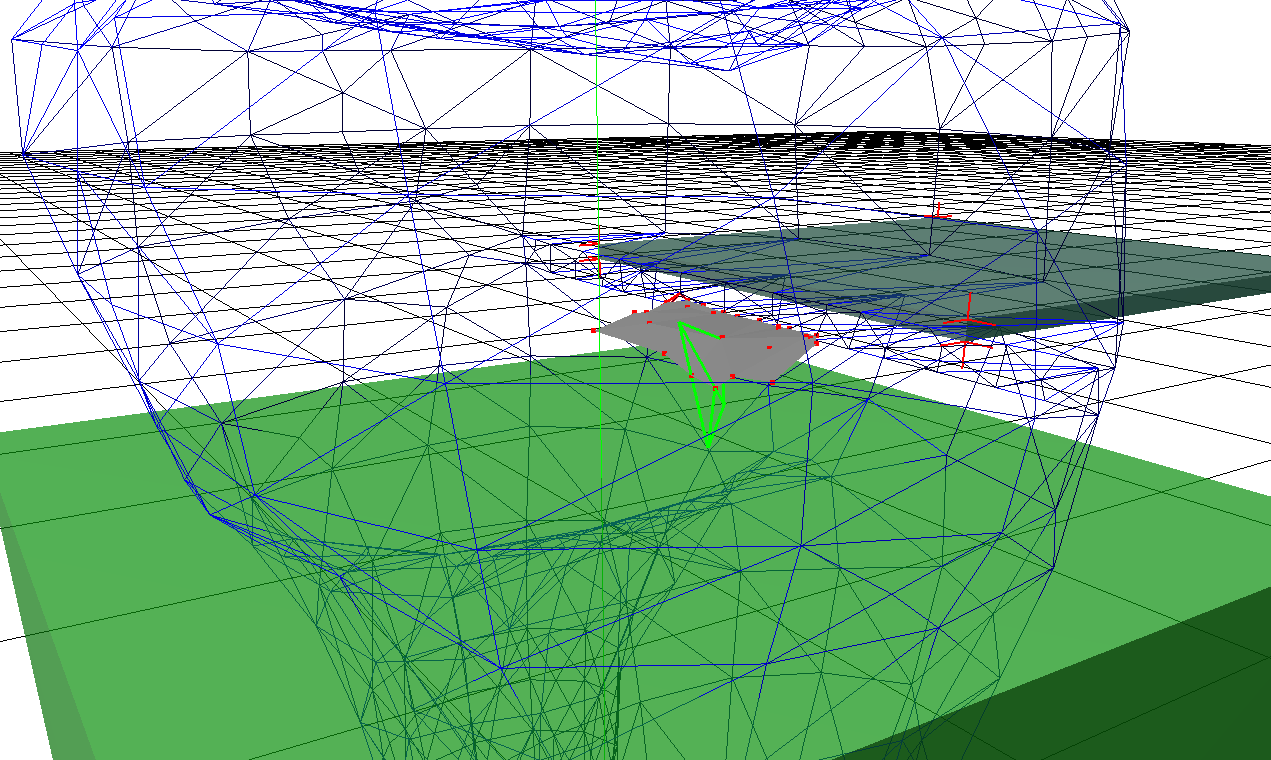
\includegraphics[width=70mm]{./images/results_tooth_fracture_propagation_1.png}
  \label{fig:tooth_crack_propagation_1}}
  \end{minipage}
  \newline
  \begin{minipage}[b]{0.5\linewidth}
    \centering
    \subfloat[]{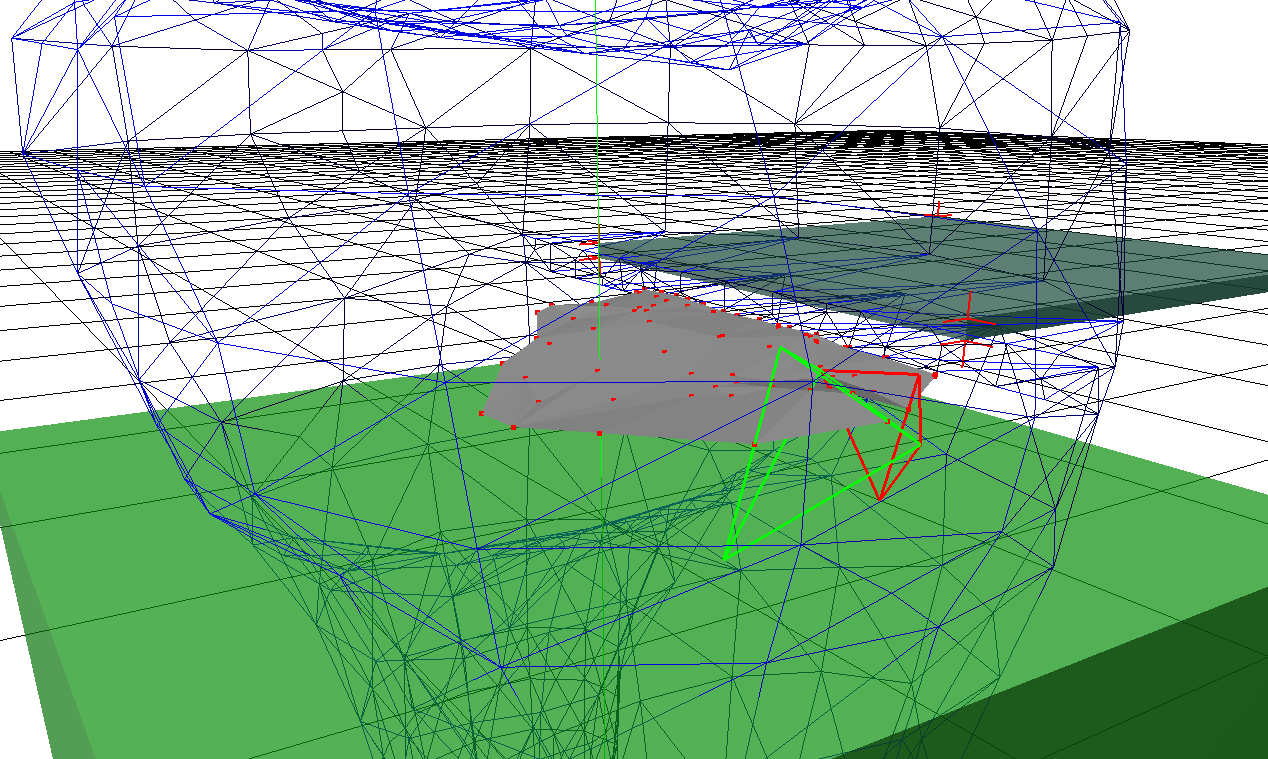
\includegraphics[width=70mm]{./images/results_tooth_fracture_propagation_2.png}
  \label{fig:tooth_crack_propagation_2}}
  \end{minipage}
%  \hspace{0.5cm}
  \begin{minipage}[b]{0.5\linewidth}
    \centering
    \subfloat[]{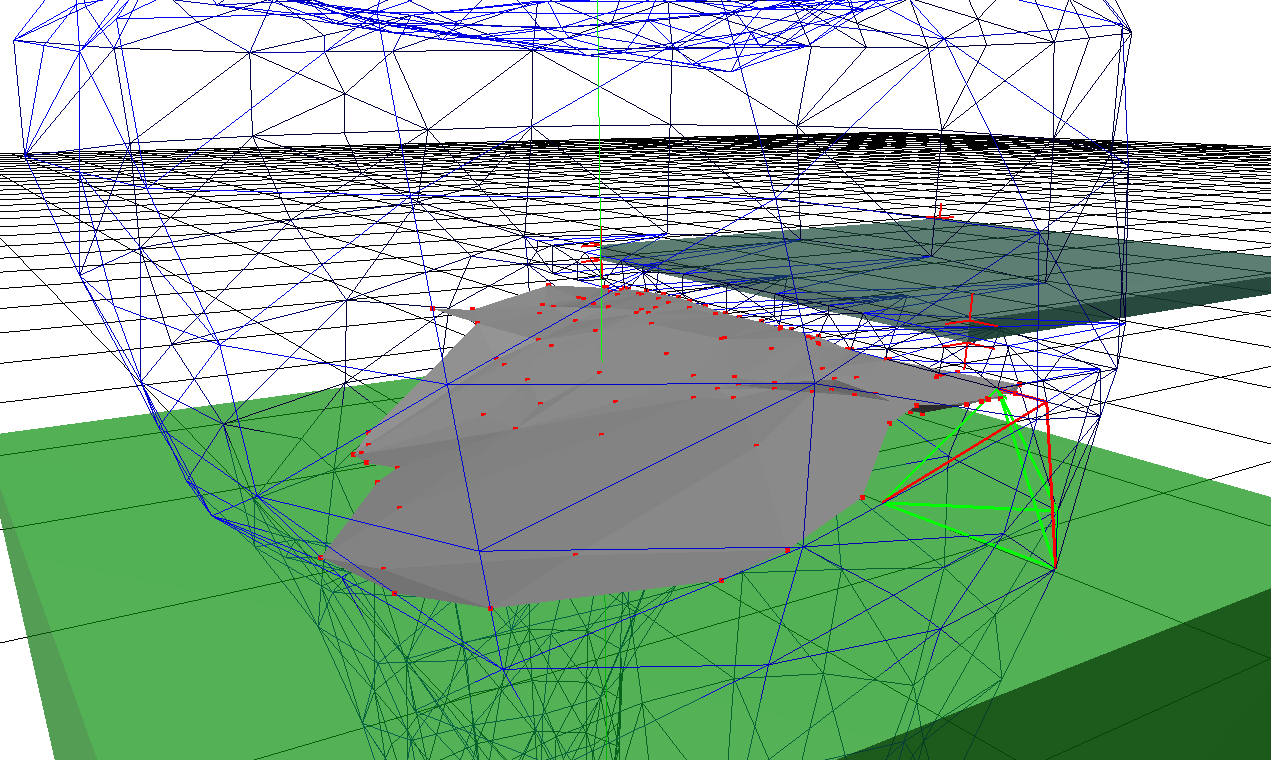
\includegraphics[width=70mm]{./images/results_tooth_fracture_propagation_3.png}
  \label{fig:tooth_crack_propagation_3}}
  \end{minipage}
  \newline
  \begin{minipage}[b]{0.5\linewidth}
    \centering
    \subfloat[]{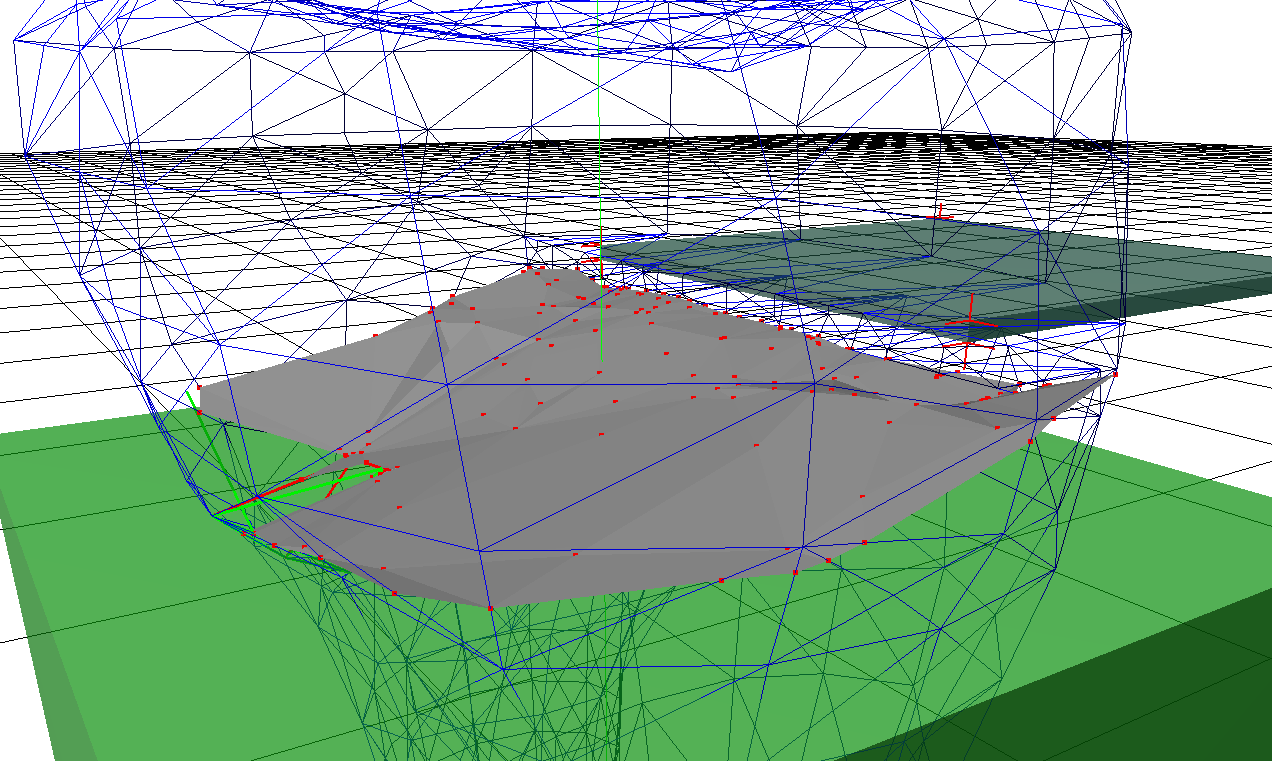
\includegraphics[width=70mm]{./images/results_tooth_fracture_propagation_4.png}
  \label{fig:tooth_crack_propagation_4}}
  \end{minipage}
 % \hspace{0.5cm}
  \begin{minipage}[b]{0.5\linewidth}
    \centering
    \subfloat[]{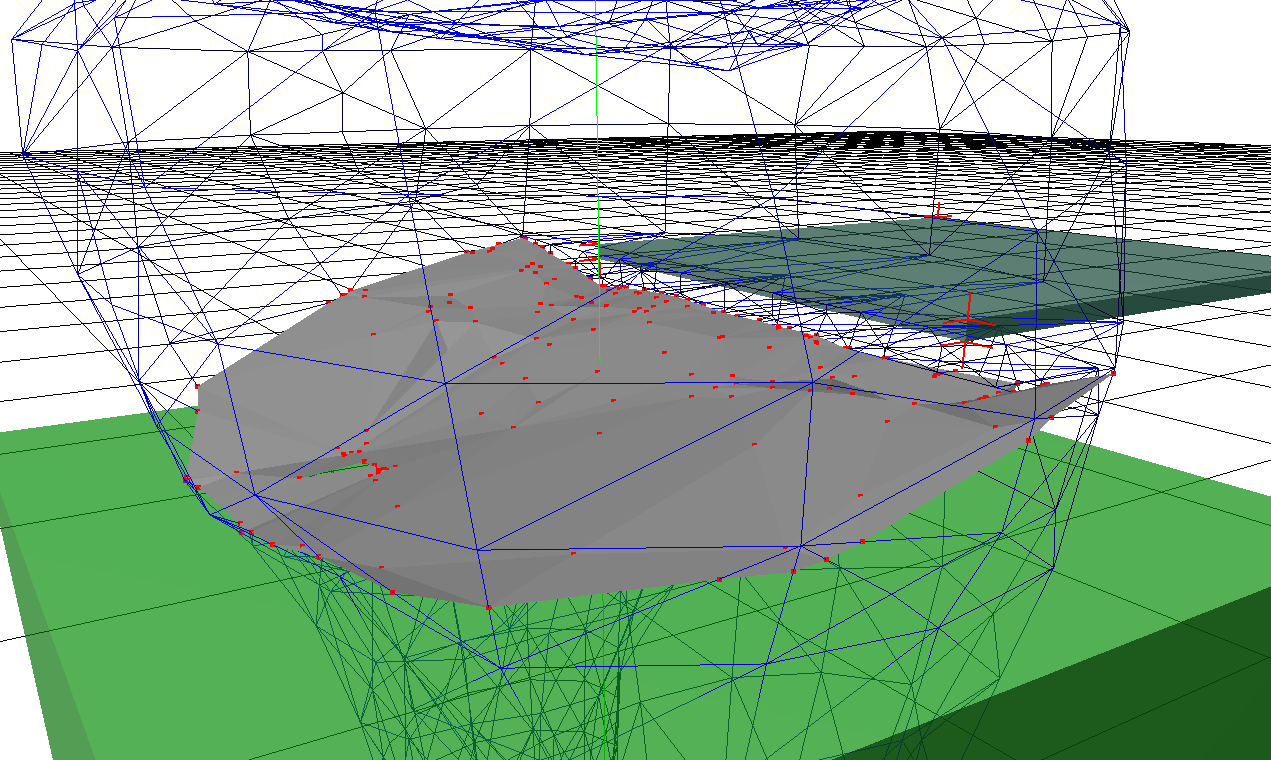
\includegraphics[width=70mm]{./images/results_tooth_fracture_propagation_5.png}
  \label{fig:tooth_crack_propagation_5}}
  \end{minipage}
  \caption{Crack propagation through tooth model.}
  \label{fig:tooth_crack_propagation}
\end{figure}


\section{Fragmentation with Varying Density}
\label{sec:fragmentation_with_varying_density}
As illustrated in section \vref{sec:realtime_analysis} we do
not have the computational resources required to perform real-time
simulation of the given model if we strictly comply with the
theoretical laws of physics.
%
Assuming the simulated model and the hardware used is unchanged, the
computational time required for performing a single iteration ($\Delta t_{sim}$) is
constant. 
%
The question is how can we increase the size of the simulated time step
without violating the boundary condition that refrains the explicit
time integration from numerical instability. We need to increase
performance at the expense of accuracy. \\


\begin{equation*}
\Delta t_{cr} = \sqrt{\frac{1}{c^2}} L_e = \alpha L_e
\end{equation*}

\begin{equation*}
\frac{1}{c^2} = \frac{\rho}{M}
\qquad \qquad
M = \frac{E(1-\nu)}{(1+\nu)(1-2\nu)}
\end{equation*}


Consider the equation for determining the critical simulated time step
$\Delta t_{cr}$. We do not wish to change the geometrical representation
of the model assuming it is reasonable, so $L_e$ is left
unchanged. The other option is to change $\alpha$ which depends on
$E$, $\nu$, and $\rho$.  If possible we do not want to 
change the elastic modulus $E$ because this would affect the relation
between stress and strain. As seen from the equations we would need to
decrease the elastic modulus to obtain a larger critical time step
hereby softening the material. Changing Poisson's ratio $\nu$ is not an
option since this only effects the contraction ratio during
deformation. With very small deformations the effect will be
minimal. Changing the density $\rho$ is an option.  
%
By increasing the density by a factor of $10^6$ we obtain a critical
time step size $\Delta t_{cr}$ of: 

% \begin{equation}
% \begin{aligned}
% \beta &= \frac{\rho}{M}
% = \frac{2580 \cdot 10^6 \frac{kg}{m^3}}{\frac{1700}{99} G \frac{N}{m^2}}
% = \frac{99 \cdot 2580 \cdot 10^6 \frac{kg}{m}}{1700 G N}
% = \frac{255420 \cdot 10^6 \frac{kg}{m}}{1700 G \frac{kg \cdot m}{s^2}}
% = \frac{255420 \cdot 10^6 \frac{1}{m}}{1700 G \frac{m}{s^2}} \\
% &= \frac{255420 \cdot 10^6}{1700 G \frac{m^2}{s^2}}
% = \frac{12771 \cdot 10^6}{85 G} \frac{s^2}{m^2}
% \approx 150.247 k^{-1} (\frac{s}{m})^2
% = 150.247 \cdot 10^{-3} (\frac{s}{m})^2
% \end{aligned}
% \end{equation}

\begin{equation}
\frac{1}{c^2} = \frac{\rho}{M}
= \frac{2580 \cdot 10^6 \frac{kg}{m^3}}{\frac{1700}{99} G \frac{N}{m^2}}
\approx 150 \cdot 10^{-3} (\frac{s}{m})^2
\qquad \wedge \qquad
\alpha = \sqrt{\frac{1}{c^2}}
\approx 387 \cdot 10^{-3} \frac{s}{m}
\end{equation}

\begin{equation}
\Delta t_{cr} = \alpha \cdot L_e
= 387 \cdot 10^{-3} \cdot 0.14 \cdot 10^{-3}
\approx 55.6 \cdot 10^{-6}s
\end{equation}

With a constant computational time of $\Delta t_{sim} = 42.6 \cdot
10^{-6}$ and a critical time step $\Delta t_{cr} = 55.6 \cdot
10^{-6}$ the real-time condition if fulfilled ( $\Delta t_{sim} \le
\Delta t_{cr}$), but how will this effect the stress and strain
behaviour and hereby the prediction of the failure surface. \\

The effect of increasing the density, besides obtaining a larger $\Delta
t_{cr}$ time step, is increased mass and damping matrices in the system due to
equation \eqref{eq:vector_component_abc} on page
\pageref{eq:vector_component_abc} where the damping factor is
determined from a constant factor $\alpha$ and the mass $M$ as $
D_{ii} = \alpha M_{ii}$.
%
The high-density object will have
increased damping but the stress and strain behaviour seems unaffected.
Recall that the rate of deformation before reaching the point of
fracture is very low in brittle materials like dentin (below $1\%$ as
calculated in section \vref{sec:results_elastic_theory}). Damping
the very limited motion has almost no effect neither on the stress and
strain nor visually.
%
The failure surface determined in the high-density material corresponds
to the failure surface determined in the material with the correct density.
Although the simulated response of the material is not theoretically
correct the failure surface in the high-density material is considered
plausible and still in correspondence with the intuition. 
In the sense of physical interpretation the change in
density is drastic and out of proportions. But in the sense of
simulated response the prediction of the crack surface seems
realistic. With the constant computational time of $42.6 \cdot 10^-6$
the stress and strain analysis is conducted about $20.000$ times pr
second facilitating real-time interaction and visualization. \\

The following test scenario illustrates how changing the density
affect the outcome of the crack tracking algorithm. The illustrations
to the left in figure \vref{fig:crack_tracking_different_density}
show the crack propagation in a tooth with the correct density
simulated in somewhat slow-motion. The illustrations to
the right are conducted with a density increase of a factor of $10^6$:

\begin{figure}
  \begin{minipage}[b]{0.5\linewidth}
    \centering
    \subfloat[]{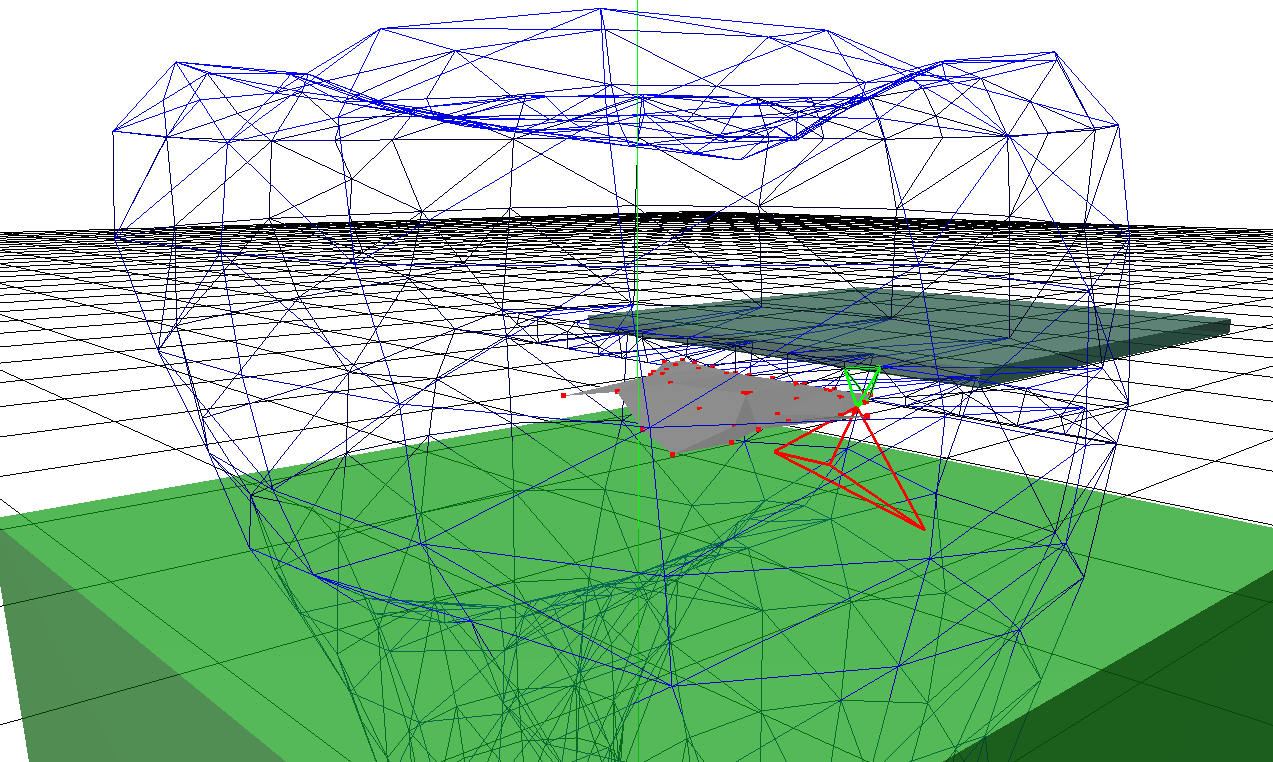
\includegraphics[width=70mm]{./images/results_density_low_0.png}
  %\label{fig:}
    }
  \end{minipage}
%  \hspace{0.5cm}
  \begin{minipage}[b]{0.5\linewidth}
    \centering
    \subfloat[]{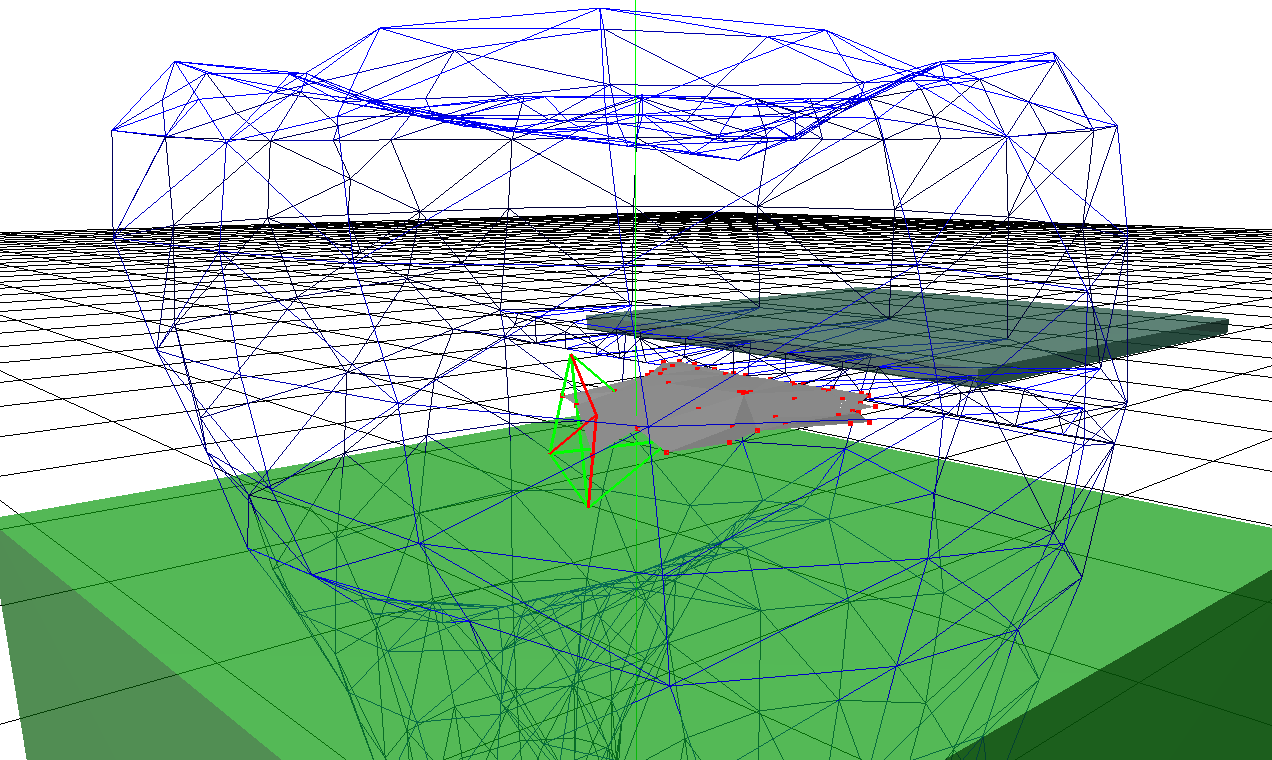
\includegraphics[width=70mm]{./images/results_density_high_0.png}
  %\label{fig:}
    }
  \end{minipage}
  \newline
  \begin{minipage}[b]{0.5\linewidth}
    \centering
    \subfloat[]{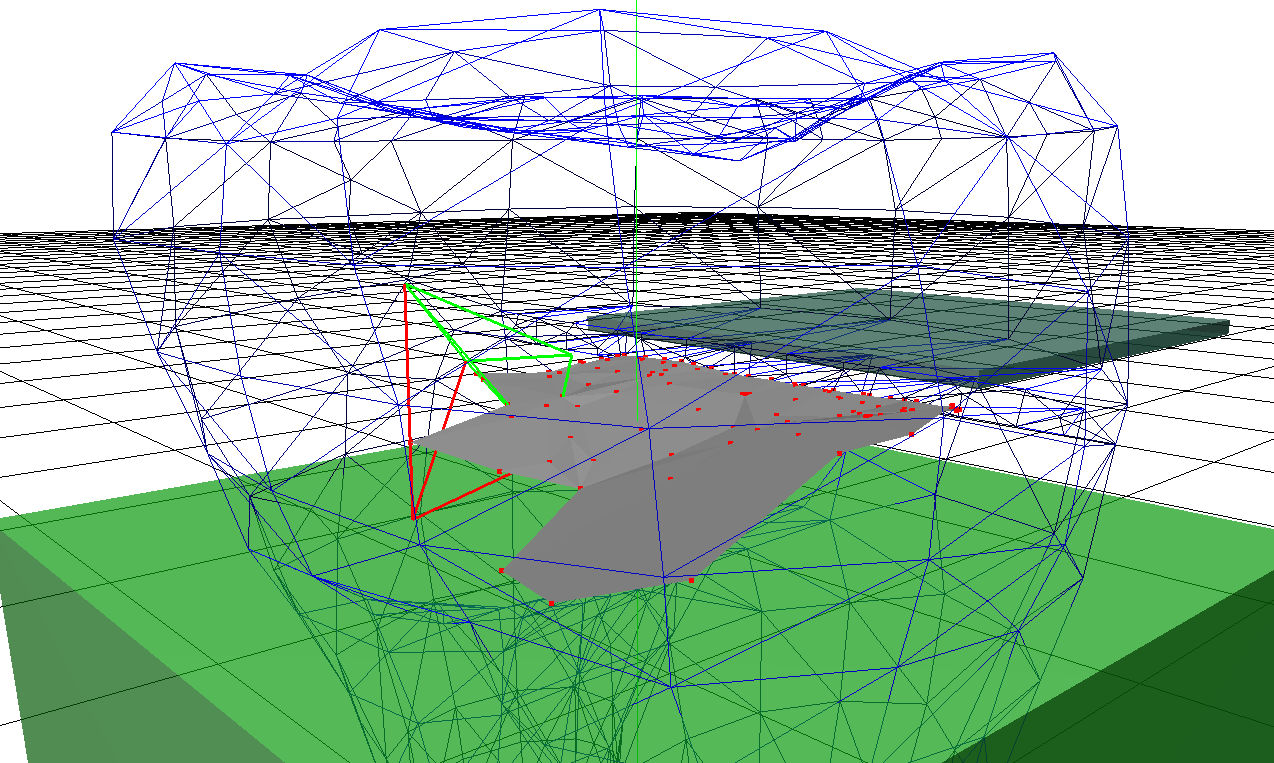
\includegraphics[width=70mm]{./images/results_density_low_1.png}
  %\label{fig:}
    }
  \end{minipage}
%  \hspace{0.5cm}
  \begin{minipage}[b]{0.5\linewidth}
    \centering
    \subfloat[]{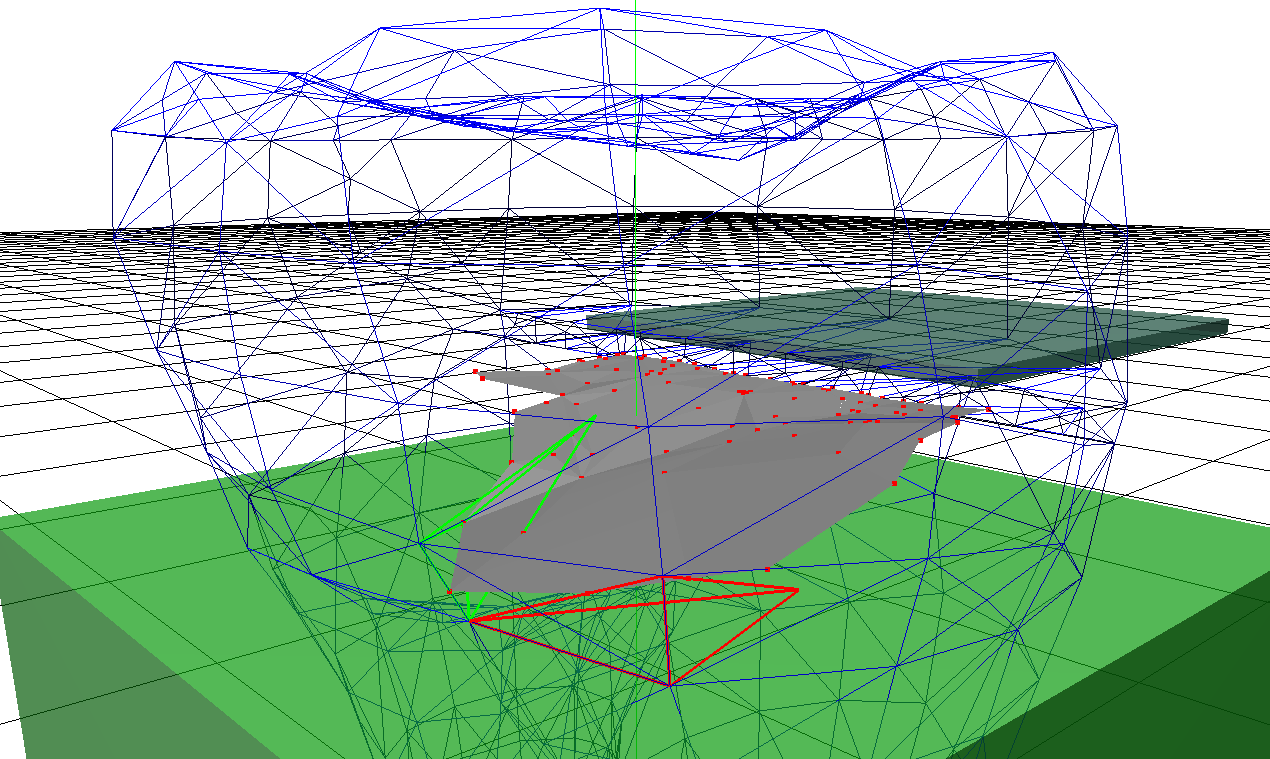
\includegraphics[width=70mm]{./images/results_density_high_1.png}
  %\label{fig:}
    }
  \end{minipage}
  \newline
  \begin{minipage}[b]{0.5\linewidth}
    \centering
    \subfloat[]{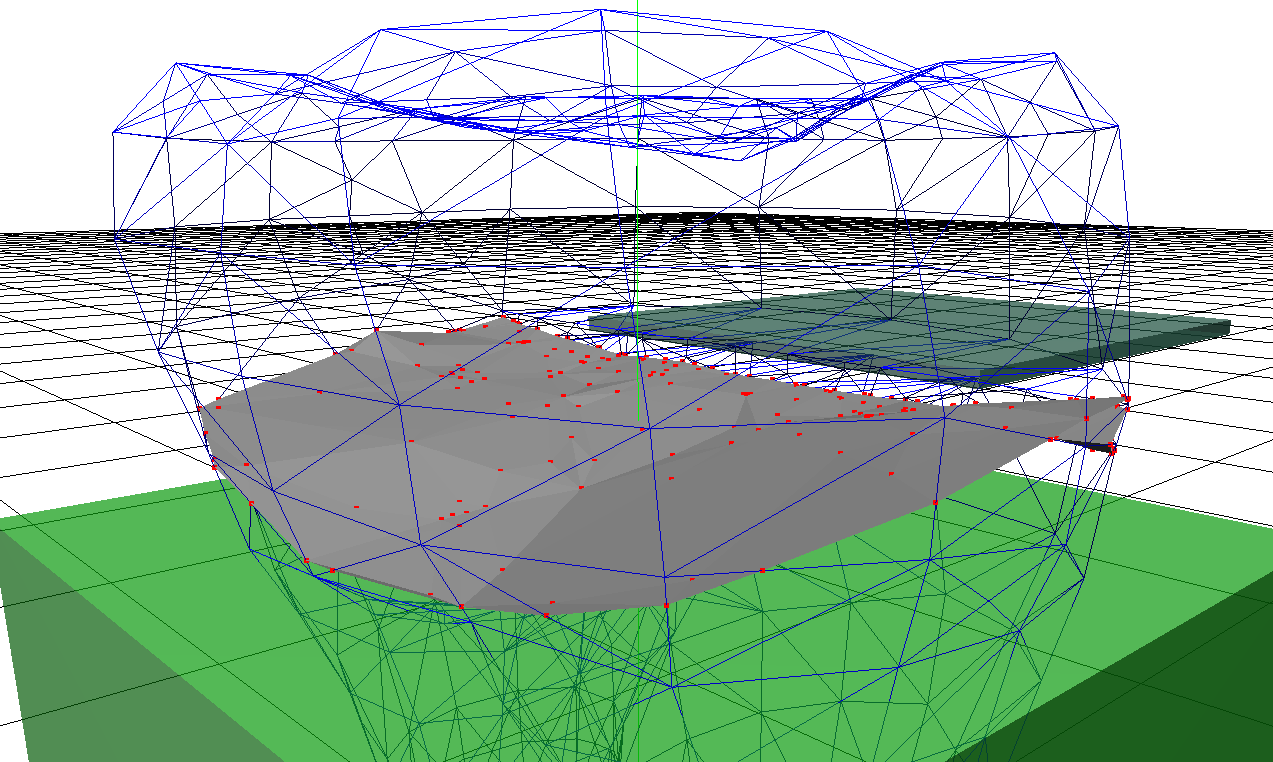
\includegraphics[width=70mm]{./images/results_density_low_2.png}
  %\label{fig:}
    }
  \end{minipage}
 % \hspace{0.5cm}
  \begin{minipage}[b]{0.5\linewidth}
    \centering
    \subfloat[]{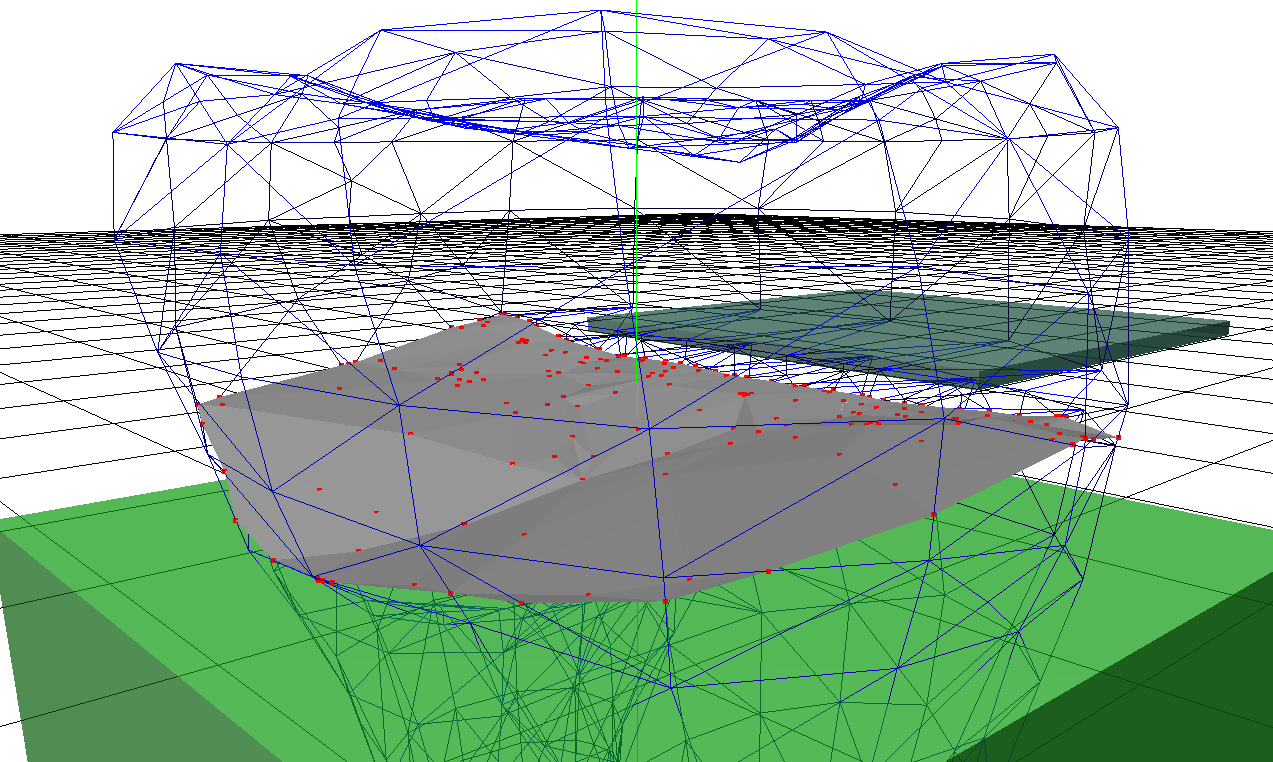
\includegraphics[width=70mm]{./images/results_density_high_2.png}
  %\label{fig:}
    }
  \end{minipage}
  \newline
  \begin{minipage}[b]{0.5\linewidth}
    \centering
    \subfloat[]{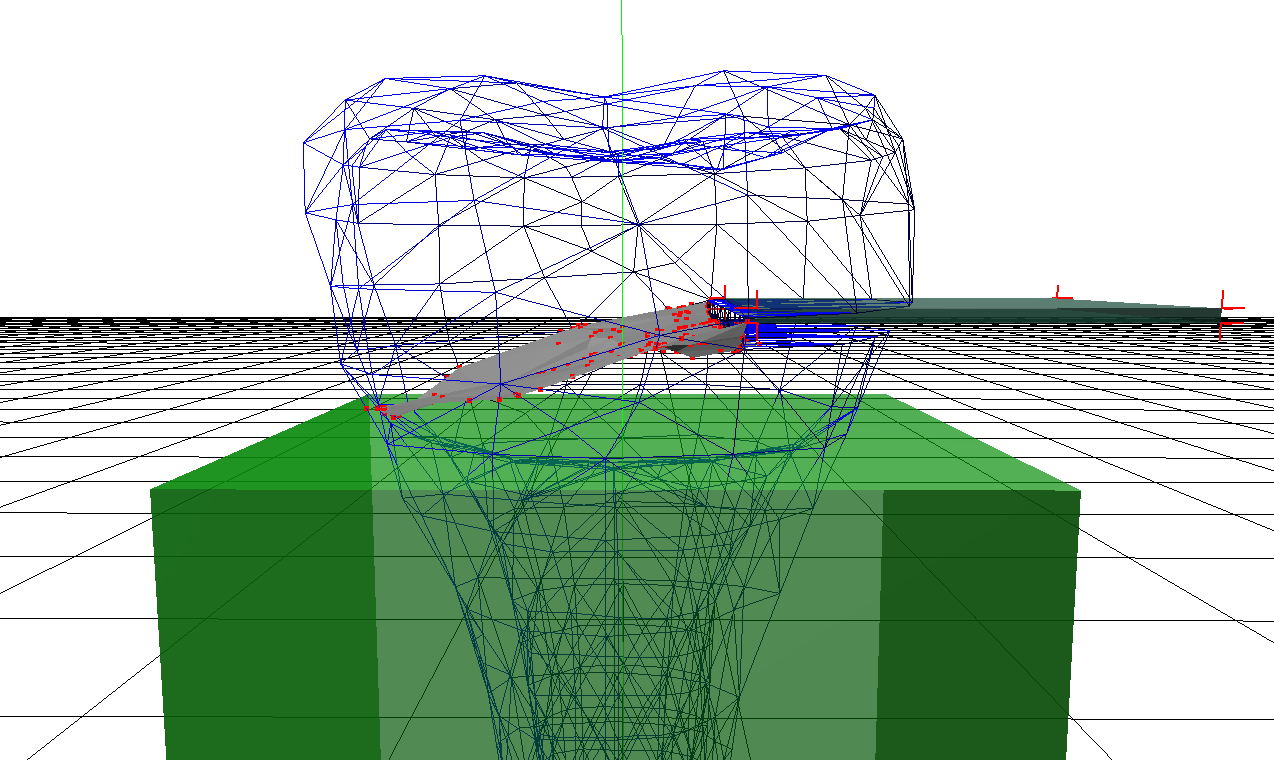
\includegraphics[width=70mm]{./images/results_density_low_3.png}
  %\label{fig:}
    }
  \end{minipage}
  %\hspace{0.5cm}
  \begin{minipage}[b]{0.5\linewidth}
    \centering
    \subfloat[]{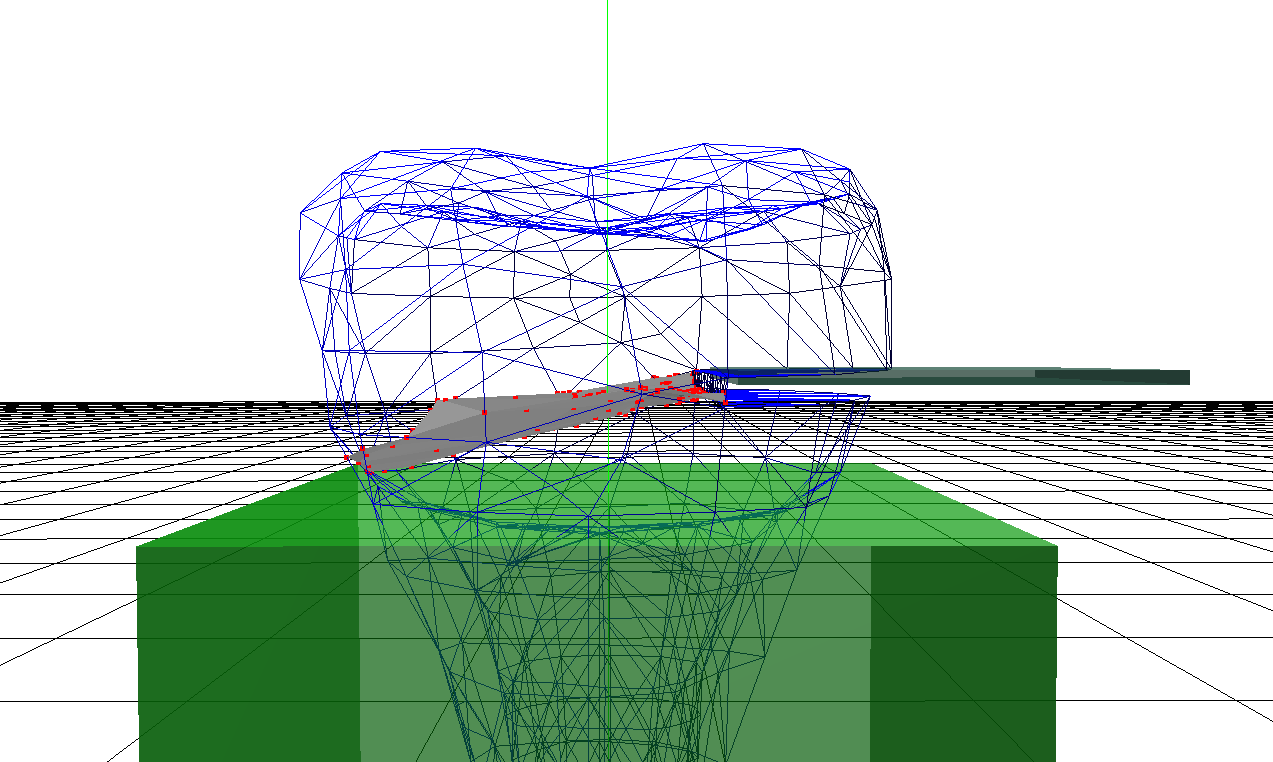
\includegraphics[width=70mm]{./images/results_density_high_3.png}
  %\label{fig:}
    }
  \end{minipage}
\caption{Crack propagation through normal contra high density material.}
\label{fig:crack_tracking_different_density}
\end{figure}


%
%
%Since the execution time $\Delta t_{sim}$ is not below the 
%
%In this case we clearly do not have that $\Delta t_{sim} < \Delta
%t_{cr}$, which means that the simulation cannot run at real-time
%frame rates.
%
%As this is precisely the simulation scenario we have constructed
%the simulator to solve, something must be done in order for us to run
%it in real-time. \newline
%
% \{
% Because we have chosen a model $\Delta t_{sim}$ cannot be changed.
% Therefore we consider the equation for calculating $\Delta t_{cr}$,
% which is a function of the minimum line segment $L_e$ in the figure
% and the material dependent constant $\alpha$.
% %
% Because we do not wish to change $L_e$, we consider $\alpha$.
% %
% Looking at the equation for $\alpha$, which we see that it is an
% function of $E$, $\nu$, and $\rho$.
% %
% And because we wish to preserve the elastic behavior of the material
% we chose to change $\rho$.
% %
% Result: $\rho$ will be multiplied by $10^6$.
% %, done effectively just be changing its unit from $kg/m^3$ to $ton/m^3$.
% \newline}
